\documentclass{article}
\usepackage{hyperref}
\usepackage[utf8]{inputenc}
\usepackage{amsfonts}
\usepackage{amsmath}
\usepackage{amssymb}
\usepackage{dsfont} % for using \mathds{1} characteristic function
\usepackage{tikz}
\usepackage{bbm}
\usepackage{relsize}
\usepackage{pgfplots}
\usepackage{scalerel}
\usepackage{wrapfig}
\usepackage[T1]{fontenc}       % change font encoding to T1
\usepackage[framed,numbered]{matlab-prettifier}
\pgfplotsset{width=10cm,compat=1.9}
\addtolength{\oddsidemargin}{-.875in}
	\addtolength{\evensidemargin}{-.875in}
	\addtolength{\textwidth}{1.75in}

	\addtolength{\topmargin}{-.875in}
	\addtolength{\textheight}{1.75in}

\usepackage{amsthm}
\definecolor{Green}{RGB}{0,210,100}
\newtheoremstyle{unnumbered} % Theorem style name
{0pt}% Space above
{0pt}% Space below
{\normalfont}% Body font
{}% Indent amount
{\bf\scshape}% Theorem head font --- {\small\bf}
{.\;}% Punctuation after theorem head
{0.2em}% Space after theorem head
{\small\thmname{#1}\thmnumber{\@ifnotempty{#1}{}\@upn{#2}}% Theorem text (e.g. Theorem 2.1)
%{\small\thmname{#1}% Theorem text (e.g. Theorem)
\thmnote{\nobreakspace\the\thm@notefont\normalfont\bfseries---\nobreakspace#3}}% Optional theorem note

\newtheoremstyle{unnumbered1} % Theorem style name
{0pt}% Space above
{0pt}% Space below
{\normalfont}% Body font
{}% Indent amount
{\bf\scshape}% Theorem head font --- {\small\bf}
{\!\!\;}% Punctuation after theorem head
{0em}% Space after theorem head
{\small\thmname{#1}\thmnumber{\@ifnotempty{#1}{}\@upn{#2}}% Theorem text (e.g. Theorem 2.1)
%{\small\thmname{#1}% Theorem text (e.g. Theorem)
\thmnote{\nobreakspace\the\thm@notefont\normalfont\bfseries---\nobreakspace#3}}% Optional theorem note

\theoremstyle{unnumbered}
\newtheorem* {theoremT}{Def}
\theoremstyle{unnumbered1}
\newtheorem* {theoremT1}{}
\RequirePackage[framemethod=default]{mdframed} % Required for creating the theorem, definition, exercise and corollary boxes
% green box
\newmdenv[skipabove=7pt,
skipbelow=7pt,
rightline=false,
leftline=true,
topline=false,
bottomline=false,
linecolor=Green,
backgroundcolor=green!0,
innerleftmargin=5pt,
innerrightmargin=5pt,
innertopmargin=5pt,
leftmargin=0cm,
rightmargin=0cm,
linewidth=2pt,
innerbottommargin=5pt]{gBox}


\newenvironment{defi}{\begin{gBox}\begin{theoremT}}{\end{theoremT}\end{gBox}}
\newenvironment{Ndefi}{\begin{gBox}\begin{theoremT1}}{\end{theoremT1}\end{gBox}}

\graphicspath{ {./images/} }

\title{Meccanica Razionale e dei Continui}
\author{Simone Paloschi}
\date{INGMTM \ \ A.A. 2022/2023}
\linespread{1.5}


\renewcommand{\contentsname}{Indice}
\begin{document}

\begin{center}
	\vspace*{1cm}
	{\Huge \textsc{Meccanica Razionale e dei Continui}}\\
	\vspace*{1cm}
	{\large {Dalle lezioni del Prof. Michele Correggi}}\\
	\vspace*{0.1cm}
	{\large per il corso di Ingegneria Matematica}\\
	\vspace*{0.7cm}
	{\large {Dispense di Simone Paloschi}}\\
	\vspace*{0.7cm}
	Politecnico di Milano\\
	A.A. 2022/2023
\end{center}
\phantom{}\\ \\

\begingroup
  \hypersetup{hidelinks}
  \tableofcontents
\endgroup


\pagebreak




%Lezione 1
\section{Cinematica}


\subsection{Cinematica del Punto Materiale}
%
\begin{Ndefi}
\textbf{Spazio delle configurazioni} di un punto materiale in $d\in\mathbb{N}$ dimensioni è lo spazio euclideo di dim d: $\mathcal{E}_d$
\end{Ndefi}
%
%
%
\textbf{Spazio vettoriale} è un insieme V con 2 proprietà: \ \ \
• : $V\times\mathbb{R}\rightarrow V$ \ \ \ \ + : $V+V\rightarrow V$ \ \ Allora:\\
\ - (V,+) è detto gruppo algebrico\\
\ - Se dimV = n allora  $\ \ \ \{\overline{u}_1,...,\overline{u}_n\}$ linearmente indipendenti è una base di V \\
\ - Data la base, \ \ $\forall \overline{z} \in V \ \ \exists! \ \alpha_1 ... \alpha_n \in\mathbb{R} \ \ t.c. \ \ \overline{z}=\sum_{j=1}^n\alpha_j\overline{u}_j$\\ \\
%
%
%
\textbf{Prodotto scalare} : $\mathbb{R}^n \times\mathbb{R}^n\rightarrow\mathbb{R}$ \ \ \ \ $\overline{u} \cdot \overline{v} \ = \ \sum^n_{j=1}u_jv_j$ \\
\textbf{Prodotto vettoriale} : $\mathbb{R}^3 \times\mathbb{R}^3\rightarrow\mathbb{R}^3$ \ \ \ \ $(\overline{u} \wedge \overline{v})_i \ = \ \sum^3_{j,k=1}\varepsilon_{ijk}\ u_jv_k$ \ \ e valgono:\\
\ • \ \ $\overline{u} \wedge \overline{v} \ = \ \
\begin{vmatrix}
\hat{i} \ \ \ \hat{j}  \ \ \ \hat{k} \\
u_1 \ u_2 \ u_3 \\
v_1 \ v_2 \ v_3 \\
\end{vmatrix}$ \\
\ • \ \ $\overline{u} \wedge \overline{v} \ = \ - \overline{v} \wedge \overline{u}$\ \ (è anticommutativo) \\
\ • \ \ $\overline{u} \wedge (\overline{v} \wedge \overline{w}) \ \neq \ (\overline{u} \wedge \overline{v}) \wedge \overline{w}$ \ \ (non è associativo)\\
\ • \ \ $\overline{u} \wedge (\overline{v} \wedge \overline{w}) \ = \ (\overline{u}\cdot\overline{w})\overline{v} - (\overline{u}\cdot\overline{v})\overline{w}$\ \ (+dim) \\
\ • \ \ $(\overline{u}+\overline{v})\wedge \overline{w} \ = \ \overline{u}\wedge \overline{w} + \overline{v}\wedge\overline{w}$ \ \ (è distributivo)  \\ \\
%
%
%
\textbf{Modulo di un vettore} : $|\overline{u}| \ = \ \sqrt{\overline{u}\cdot\overline{u}} $ \ \ valgono: \\
\ • \ \ $\overline{u}\cdot\overline{v} = |\overline{u}||\overline{v}|cos\theta $ \\
\ • \ \ $\overline{u}\wedge\overline{v}=|\overline{u}||\overline{v}|sen\theta$ \\ \\
%
%
%
\textbf{Spazio euclideo} $\mathcal{E}_d$ è un insieme di punti $\mathcal{E}_d$ e un'applicazione A: $\mathcal{E}_d\times\mathcal{E}_d\rightarrow V$ (spazio vettoriale) t.c. \\
%
\ • \ \ $P,Q \in\mathcal{E}_d \rightarrow \overline{PQ}\in V$ \ \ \ \ \ \ • \ \ $\overline{PQ}=-\overline{QP}$ \\
\ • \ \ $\overline{PQ}+\overline{QR}=\overline{PR}$ \ \ \ \ \ \ \ \ \ \ \ \ • \ \ $\forall P \in \mathcal{E}_d, \forall \overline{u} \in V \ \ \exists! \ Q \in \mathcal{E}_d \ | \ \overline{PQ}=\overline{u}$ \\
%
%
%
\begin{defi}
Un \textbf{osservatore}, o sistema di riferimento, in $\mathcal{E}_d$ è un insieme: $\mathcal{O}= \{O; \hat{e}_1,...,\hat{e}_d \}$ t.c.

$O\in\mathcal{E}_d$ e $ \{\hat{e}_1,...,\hat{e}_d \} $ è un sistema ortonormale in $\mathbb{R}^d$
\end{defi}
%
La configurazione del punto materiale P si può assegnare con le \textbf{coordinate} $\overline{n} \in\mathbb{R}^d$ di P rispetto a $\mathcal{O}$ \\
Le coordinate $\overline{x}(t)$ di P rispetto al tempo si possono vedere come:\\
\ • \ \ punto nello spazio-tempo $\mathbb{R}^d\times\mathbb{R}$ che individua la linea di universo di P \\
\ • \ \ funzione $\overline{x}(t): \mathbb{R}\rightarrow\mathbb{R}^d$ è detta \textbf{traiettoria} \ (o moto) \\
%
\begin{defi}
Data la traiettoria e assunta $\overline{x}(\cdot) \in C^2(\mathbb{R})$ \ \ \ 
\textbf{velocità}: $\overline{v}(t) = \frac{d\overline{x}}{dt}(t)$ \ \ \ \ \textbf{accelerazione}: $\overline{a}(t) = \frac{d^2\overline{x}}{dt^2}(t)$
\end{defi}

\pagebreak %se lo togli metti \\



%Lezione 2
\subsection{Moto in Coordinate Intrinseche}
%
\begin{Ndefi}
Sia $\overline{x}(\cdot) \in C^2([t_0,t_1])$ la traiettoria di P. \ Assumendo che $\overline{x}(t)$ abbia solo zeri isolati allora: \\ 
l'\textbf{ascissa curvilinea} è la lunghezza dell'arco di curva percorsa tra $t_0$ e t: \ \ $s(t)=\int_{t_0}^t \dot{s}(\tau) d\tau \ = \ \int_{t_0}^t |\dot{\overline{x}}(\tau)| d\tau$
\end{Ndefi}
%
Oss: s(t): $\mathbb{R}\rightarrow\mathbb{R}^+$ anche detta legge oraria del moto del punto, è una funzione monotona crescente.\\
%
\phantom{Oss: }di conseguenza s($\cdot$) è invertibile $\implies \exists \ t(\cdot):\mathbb{R}^+\rightarrow\mathbb{R}$ \ t.c. \ s(t($\sigma$)) = $\sigma$ \ e \ $\frac{dt}{ds}(s)= \frac{1}{|\dot{\overline{x}}(t(s))|}\ \ \ \forall t \ |\ \overline{v}(t)\neq \overline{0} $\\
Oss: Possiamo quindi parametrizzare ugualmente le curve con il tempo o con la distanza percorsa\\
Notazione: $\dot{f}=\frac{df}{dt} \ \ f'=\frac{df}{ds}$ \\ \\
%
%
%
Poste le ipotesi su $\overline{x}(\cdot)$ sono definiti la parametrizzazione $\overline{\gamma}:[0,L]\rightarrow\mathbb{R}^d$ t.c. $\overline{\gamma}(s)=\overline{x}(t(s))$ e i versori:
\ • \ \ \textbf{tangente} \ \ $\hat{\tau}(s) := \overline{\gamma}'(s) $ \\
\ • \ \ \textbf{normale} \ \ $\hat{n}(s):=\frac{\hat{\tau}'(s)}{|\hat{\tau}'(s)|}$\\
\ • \ \ \textbf{binormale} \ \ $\hat{b}(s):=\hat{\tau}(s)\wedge\hat{n}(s)$ \\
Inoltre possiamo definire i seguenti valori: \\
\ • \ \ \textbf{curvatura} della traiettoria \ \ $k:[0,L]\rightarrow\mathbb{R}^+$ \ t.c. \ $k(s) := |\hat{\tau}'(s)|$\\
\ • \ \ \textbf{torsione} della curva \ \  $h:[0,L]\rightarrow\mathbb{R}^+$ \ t.c. \ $h(s) := |\hat{b}'(s)|$ \\ \\
%
%
%
Teorema: \ \textbf{Formule di Frenet-Serret} \ \ \ (+dim)\\
\phantom{\ } Sotto le ipotesi di $\overline{x}(\cdot)$ e $\forall s \in [0,L] \ t.c. \ \overline{\gamma}'(s)\neq 0$ \\
\ • \ $\hat{\tau}(s), \hat{n}(s), \hat{b}(s)$ formano una terna ortonormale in $\mathbb{R}^3$ \ \ \ \ \ \ • \
$\begin{cases}
\hat{\tau}'(s)=k(s)\hat{n}(s) \\
\hat{n}'(s)=-k(s)\hat{\tau}(s)+h(s)\hat{b}(s)\\
\hat{b}'(s)=-h(s)\hat{n}(s)
\end{cases}$ \\ \\
Prop: Poste le ipotesi su $\overline{x}(\cdot)$ si ha: \ \ \ \
• $\overline{v}(t)=\dot{s}(t)\hat{\tau}$ \ \ \ \
• $\overline{a}(t)=\ddot{s}(t)\hat{\tau}+k\dot{s}^2(t)\hat{n}$ \ \ \ (+dim)\\




\subsection{Cinematica del Corpo Rigido}
%
\begin{defi}
Un \textbf{corpo rigido} è un sistema di $N\in\mathbb{N}\cup\{+\infty\}$ punti materiali che soddisfano: \\ $|\overline{OP}_i(t) - \overline{OP}_j(t)|$ = cost   $\forall t \in \mathbb{R} \ \ \forall i,j \in \{1...N\}$ 
\  ovvero la distanza tra i punti del sistema rimane costante\\
Per identificare univocamente la configurazione del corpo rigido in 3D per N$\ge$3 servono 3N-6 coordinate.
\end{defi}
%
%Lezione 3
%
\begin{defi}
Un osservatore, o anche sistema di riferimento, è \textbf{solidale} ad un corpo rigido se le posizioni del corpo rispetto a $\theta = \{O',\hat{e}_1, \hat{e}_2, \hat{e}_3 \} $ non dipendono dal tempo.
\end{defi}
%
Teorema: Un sistema di punti materiali è un corpo rigido se e solo se $\exists \theta$ solidale \ \ \ (+dim) \\
%
Oss: La posizione di un punto nello spazio è assegnata univocamente dalle distanze da 3 punti non collineari. \\ \\
%
Prop: La configurazione di un corpo rigido piano è determinata univocamente da 3 coordinate\ \ \ \ (+dim)\\
%
Prop: Per la configurazione di un C tridimensionale sono necessarie e sufficienti 6 coordinate \ \ \ \ (+dim)\\ \\
%
%
%
Prop: Ogni rotazione in $\mathbb{R}^3$ è rappresentata da una matrice ortonormale $R\in\Theta_3$, \\
\phantom{Prop: }Che equivale al prodotto di 3 rotazioni attorno agli assi $\hat{i}, \hat{j}, \hat{k}$. \ \ \ \ \ \ \ \ \ \ \ \ \ \ \ \ \ \ \ \ \ \ \ \ \ \ \ \ \ \ \ \ \ \ \ \ \ \ \ \ \ \ \ \ \ \ \ \ \ \ \ \
%
%
%
\begin{wrapfigure}{r}{0.16\textwidth}
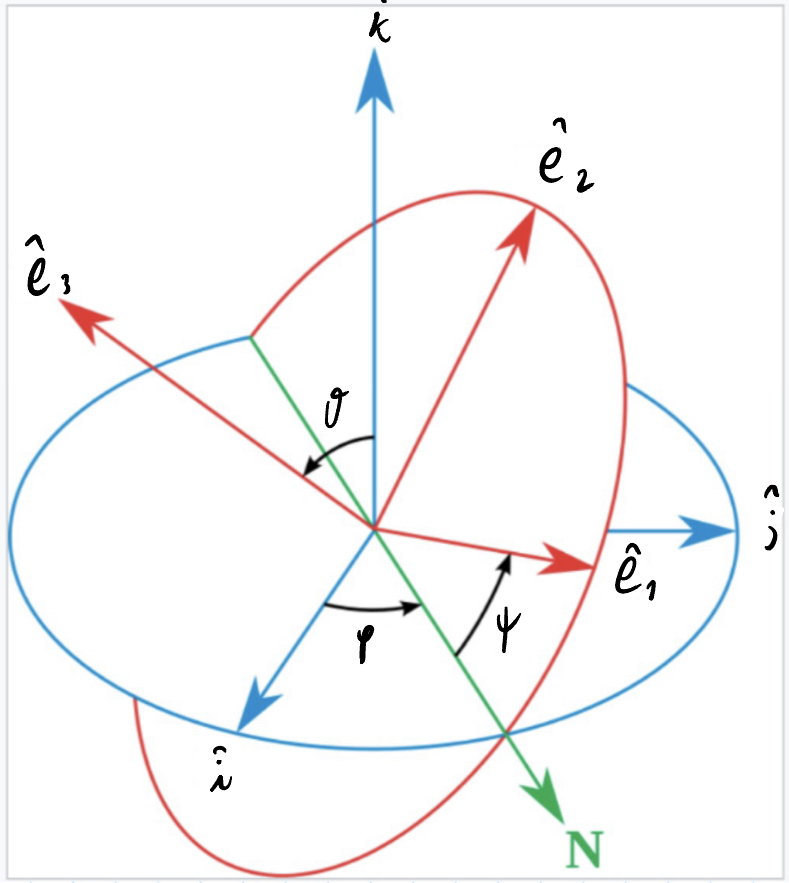
\includegraphics[width=0.16\textwidth]{Eulero.jpeg}
\end{wrapfigure}\\
%
%
Gli \textbf{Angoli di Eulero} sono coordinate angolari che identificano univocamente 

la posizione di un sistema solidale, nell'ipotesi O=O':\\
%
%
\ • \ \ $\theta$ angolo di \textbf{mutazione} $\in [0,\pi]\ :\ cos\theta := \hat{e}_3\cdot\hat{k}$; \\
\ • \ \ $\phi$ angolo di \textbf{precessione} $\in [0,2\pi]\ :\ cos\phi := \hat{i}\cdot\frac{\hat{k}\wedge\hat{e}_3}{|\hat{k}\wedge\hat{e}_3|}$; \\
\ • \ \ $\psi$ angolo di \textbf{rotazione propria} $\in [0,2\pi]\ :\ cos\psi := \hat{e}_1\cdot\frac{\hat{k}\wedge\hat{e}_3}{|\hat{k}\wedge\hat{e}_3|}$; \\
\phantom{}\\
%
%
%
Prop: Vale sempre, per un corpo rigido: \ $(\overline{V}_P-\overline{V}_Q)\cdot\overline{QP} = 0$ \ \ \ dove \ $\overline{QP}=\overline{X}_P-\overline{X}_Q$ \\
\phantom{}\\
%
%
%
Teorema: Poisson \ \ \ \ (+dim)\\
\phantom{\ } Dato un corpo rigido C e una terna ortonormale solidale, $\exists! \ \overline{\omega} \in \mathbb{R}^3$ detta \textbf{velocità angolare} t.c. \\
\phantom{} \hspace{2in} $ \dot{\hat{e}}_j = \overline{\omega}\wedge\hat{e}_j \ \ \ \ \ \forall j \in \{1,2,3\}$ \\
%
%
%
Teorema: formula fondamentale della cinematica rigida\ \ \ (+dim)\\
\phantom{\ } Per ogni corpo rigido C, $\exists! \ \overline{\omega} \in \mathbb{R}^3$ detta velocità angolare t.c. \\
\phantom{} \hspace{1.4in} $\overline{V}_P(t)-\overline{V}_Q(t) = \overline{\omega}(t)\wedge\overline{QP}(t) \ \ \ \ \ \forall P,Q \in C \ \ \forall t \in \mathbb{R}$ \\
%
%Lezione 4
%
\begin{defi}
Il \textbf{moto} di un corpo rigido C è: \\
\ • \ \ \textbf{traslatorio} se $\overline{V}_P = \overline{V}_Q \ \ \forall P,Q \in C$ \\
\ • \ \ \textbf{piano} se \ \ \ \ $\begin{cases} 
\exists \hat{k} \in \mathbb{R}^3 \ t.c. \ \overline{V}_P(t) \perp \hat{k} \ \ \forall P\in C \ \forall t\in\mathbb{R} \\
\overline{PQ}(t) /\!\!/ \hat{k} \implies \overline{V}_P(t) = \overline{V}_Q(t)  \end{cases}$ \\
\ • \ \ \textbf{polare} se $\exists$ \textbf{polo} $O \in C$ t.c. $\overline{V}_O(t)=\overline{0} \ \ \forall t$ \\
\ • \ \ \textbf{rotatorio} se $\exists$ \textbf{asse di rotazione} r t.c. $\forall P \in r \ \overline{V}_P(t) = \overline{0} \ \forall t$ \\
\ • \ \ \textbf{rototraslatorio} se è una combinazione di un moto rotatorio e uno traslatorio
\end{defi}
%
%
%
Un corpo rigido è \textbf{piano} se $\exists \hat{k} \in \mathbb{R}^3 \ t.c. \ \overline{x}_j \perp \hat{k} \ \forall j \in C$ \\ \\
%
%
%
Prop: Moto di un corpo rigido è traslatorio $\Longleftrightarrow \overline{\omega}(t) =0 \ \ \forall t \in \mathbb{R}$ \ \ \ (+dim) \\
Prop: Moto di un corpo rigido è rototraslatorio $\Longleftrightarrow \overline{\omega}(t) = \omega(t)\hat{k}$ con $\hat{k}$ costante \ \ \ (+dim) \\
Lemma: Moto di un corpo rigido è rototraslatorio $\Longleftrightarrow \exists \ \hat{e}_j$ solidale t.c. $\dot{\hat{e}}_j=0$ \ \ \ (+dim) \\ \\
Oss: • Un moto traslatorio non è necessariamente rettilineo \ \ • l'asse di rotazione r ha equazione: $\overline{x}=\lambda\hat{k} + \overline{z}(t)$ \\
Prop: Un moto rigido è piano $\Longleftrightarrow \begin{cases}
\exists \hat{k} \in \mathbb{R}^3 \ t.c. \ \overline{\omega}(t)= \omega(t)\hat{k} \\
\exists Q \in C \ t.c. \ (\overline{x}_Q(t)-\overline{
x}_Q(0))\cdot \hat{k} = 0 \ \ \forall t \in \mathbb{R} \end{cases}$ \ \ \ (+dim) \\ 
Corollario: Ogni moto rigido piano è rototraslatorio \\
%
%
%
\begin{defi}
L'\textbf{atto di moto} di un sistema di punti materiali al tempo t è: $A(t)=\{ (\overline{x}_j(t),\overline{v}_j(t)), j\in\{1,..,N\} \}$
\end{defi}
\ • \ \ \textbf{traslatorio} \ \ se $\overline{v}_i=\overline{v}_j \ \ \forall i,j \in \{1,...,N\}$ \\
\ • \ \ \textbf{piano} \ \ se $\begin{cases}
\exists \hat{k} \in \mathbb{R}^3 \ t.c. \ \overline{v}_j \perp \hat{k} \ \ \forall j \in \{1,...,N\} \\
se \ (\overline{x}_i -\overline{x}_j) /\!\!/ \hat{k} \implies \overline{v}_i = \overline{v}_j \end{cases}$ \\
\ • \ \ \textbf{rigido} \ \ se è compatibile con il vincolo di rigidità \\
\ • \ \ \textbf{rototraslatorio} \ \ se $ \exists \hat{e} \ t.c. \ \ \forall P,Q \in C \ con \ \overline{PQ} /\!\!/ \hat{e} \implies \overline{v}_P = \overline{v}_Q$ \\
\ • \ \ \textbf{elicoidale} \ \  se è rototraslatorio ed $\exists \ r: \overline{x}=\lambda\hat{e} + \overline{z} \ con \ \overline{v}_P = \overline{v}_Q = \mu \hat{e} \ \ \forall P,Q \in r\cap C$\\
\ • \ \ \textbf{rotatorio} \ \ se è rototraslatorio e $\exists$ asse di istantanea rotazione $ \ r_{ir}: \overline{x}=\lambda\hat{e} + \overline{z} \ \ \ t.c. \ \overline{v}_P = \overline{0} \ \ \ \forall P\in r_{ir} \cap C \ $ \\
%
Prop: Ogni atto di moto rigido è rototraslatorio \ \ \ (+dim)\\
%
%
%
\begin{defi}
L'\textbf{invariante scalare} di un atto di moto rigido è la quantità $I=\overline{\omega}\cdot\overline{v}_P$ con P $\in C$
\end{defi}
Oss: $I$ non dipende dalla scelta di P per la formula cinematica rigida: $\overline{\omega}\cdot\overline{v}_Q = \overline{\omega}\cdot(\overline{v}_P+\overline{\omega}\wedge\overline{PQ})=\overline{\omega}\cdot\overline{v}_P$\\ \\
%
%Lezione 5
%
Teorema: Mozzi \ \ \ (+dim) \\
\phantom{\ }Un atto di moto rigido di velocità angolare $\overline{\omega}$ è:\\
\ • \ \ traslatorio $\Longleftrightarrow \overline{\omega}=\overline{0}$ \\
\ • \ \ rotatorio $\Longleftrightarrow \overline{\omega} \neq \overline{0}$ e $I=0$, in tal caso l'asse di istantanea rotazione è $r_{ir}: \overline{x}=\lambda\overline{\omega} + \frac{\overline{\omega} \wedge \overline{v}_P}{|\overline{\omega}|^2}+\overline{x}_p $ \\
\ • \ \ elicoidale $\Longleftrightarrow \overline{\omega} \neq \overline{0} $ e $I\neq0$, in tal caso l'asse di mozzi è $r_{mozzi}: \overline{x}=\lambda\overline{\omega} + \frac{\overline{\omega} \wedge \overline{v}_P}{|\overline{\omega}|^2}+\overline{x}_p $\\
\phantom{\ }L'\textbf{asse di mozzi} ha le seguenti proprietà: \ \
i) $\overline{v}_P /\!\!/ \overline{\omega} \ e\ \overline{v}_P = \frac{I\overline{\omega}}{|\overline{\omega}|^2} \ \ \forall P \in r_{mozzi}$ \\
\phantom{\ }ii) $|\overline{v}_P|$ è minima in C se $P \in r_{mozzi}$ \hspace{0.42in}
iii) se $\overline{PQ} /\!\!/ r_{mozzi} \implies \overline{v}_P = \overline{v}_Q$ \\ \\
%
%
%
Oss: Ogni atto di moto rotatorio è anche piano con $\hat{k}=\frac{\overline{\omega}}{|\overline{\omega}|}$ \\
Corollario: Ogni atto di moto rigido piano è
\ \ • \ traslatorio $\Longleftrightarrow \overline{\omega}(t)=\overline{0}$
\ \ • \ rotatorio $\Longleftrightarrow \overline{\omega}(t) \neq \overline{0}$
\begin{defi}
Il \textbf{centro di istantanea rotazione} è il punto t.c. $r_{ir} \cap \Pi = \{CIR\}$ con $\Pi$ il piano del moto
\end{defi}
%
Oss: In un atto di moto rigido piano la posizione del CIR identifica univocamente l'atto di moto
%
%
\begin{wrapfigure}{r}{0.16\textwidth}
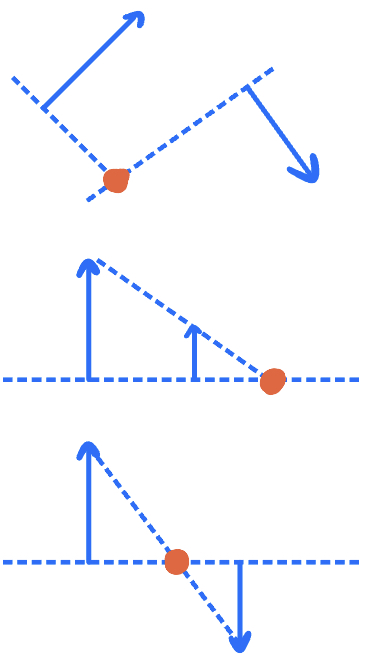
\includegraphics[width=0.18\textwidth]{CIR.jpeg}
\end{wrapfigure}

\phantom{\ \ \ }  Inoltre il CIR può anche essere fuori dal corpo rigido \\ \\
%
%
%
Teorema: Chasles \ \ \ (+dim)\\ 
\phantom{\ }La posizione del CIR in un atto di moto rigido piano si trova: \\
\ \ • \ all'intersezione delle rette perpendicolari a $\overline{v}_P \ e\ \overline{v}_Q$ passanti per P e Q \\
\ \ • \ sulla retta $\perp \ a \ \overline{v}_P /\!\!/ \overline{v}_Q$ t.c. $\frac{|\overline{v}_P|}{|\overline{CP}|} = \frac{|\overline{v}_Q|}{|\overline{CQ}|}$ \\
\pagebreak




\subsection{Cinematica Relativa}
%
%
Prop: Trasformate di Galileo (o legge di trasformazioni della velocità) \ \ \ (+dim)\\
\phantom{\ } $\exists$ matrice ortogonale $R\in\theta_3 \ t.c \ \overline{x}_P = R\overline{x}_P' + \overline{OO'}$ e un vettore $\overline{\omega} \in \mathbb{R}^3$ t.c. \\
\phantom{\ } $\overline{v}_P = \overline{v}_P' + \underline{ \overline{v}_{O'} + \overline{\omega} \wedge \overline{x}_P'}$ \ \ \ dove $\overline{v}_{O'}$  è velocità relativa e \underline{ \ \ }  è velocità di trascinamento \\ \\
%
%Lezione 6
%
Teorema: Coriolis \ \ \ (+dim)\\
\phantom{\ } Dati due osservatori $\theta \ e \ \theta'$ con accelerazione relativa $\overline{a}_{O'}$ e velocità angolare $\omega$, allora: \\
\phantom{} \hspace{1in} $\overline{a}_P=\overline{a}_P' +  \underline{\overline{a}_{O'} + \dot{\overline{\omega}}\wedge\overline{x}_P' +  \overline{\omega}\wedge(\overline{\omega}\wedge\overline{x}_P')} +  2\overline{\omega}\wedge\overline{v}_P'$ \\
\phantom{\ } dove \underline{ \ \ } è l'accelerazione di trascinamento, \ \ $\overline{\omega}\wedge(\overline{\omega}\wedge\overline{x}_P')$ è l'acc. centrifuga \ e \ $2\overline{\omega}\wedge\overline{v}_P'$ è l'acc. di Coriolis \\ \\
%
%
%
Oss: Affinché $\theta \ e\ \theta'$ abbiano le stesse accelerazioni $(\overline{a}_P = \overline{a}_P')$,  serve \ $\overline{a}_{O'}=\overline{\omega}=\dot{\overline{\omega}}=\overline{0} $ \\
\phantom{Oss: }allora $\theta \ e\ \theta'$ sono osservatori relativamente inerziali e sono in moto relativo rettilineo uniforme \\
%
%
Corollario: Rivals \ \ \ (+dim)

Dati P e Q di un corpo rigido si ha \ \ $\overline{a}_P=\overline{a}_Q + \dot{\overline{\omega}}\wedge\overline{QP} +  \overline{\omega}\wedge(\overline{\omega}\wedge\overline{QP})$ \\
%
%
Corollario: Dato un corpo rigido con $\overline{\omega}, \dot{\overline{\omega}}\neq\overline{0},$

$\exists! C$ centro delle accelerazioni t.c. $\overline{a}_C = \overline{0} \ e \ \forall P \in C \ \ \ \overline{PC} = \frac{  \dot{\overline{\omega}}\wedge\overline{a}_P - \overline{\omega}\wedge(\overline{\omega}\wedge\overline{a}_P) }{ \omega^4 + \dot{\omega}^2  } $ \\




\subsection{Moti e Atti di moto Rigidi}
%
%
%
Riassunto Moti piani:\\
\ • \ \ Traslatorio ha atto di moto traslatorio $\forall t$\\
\ • \ \ Rotatorio, Rototraslatorio, Polare hanno atto di moto rotatorio $\forall t$\\
Per gli atti di moto rotatorio piani abbiamo: $\begin{cases}
\overline{\omega}(t)=\dot{\theta}\hat{k} \\
\overline{V}_P=\overline{\omega}(t)\wedge\overline{CP}
\end{cases}$ \\ \\
%
%
%
Prop: Composizione velocità angolari \ \ \ (+dim)\\
\phantom{Prop: }Siano $\overline{\omega}_C, \ \overline{\omega}_C' \ e \ \overline{\omega}$ le velocità angolari di C rispetto a $\theta \ e\ \theta'$ e di $\theta'$ rispetto a $\theta$, allora: \ \ \ $\overline{\omega}_C = \overline{\omega}_C' + \overline{\omega}$ \\
Oss: Questa legge può essere utile per decomporre, con osservatori mobili, il moto in moti più semplici
%
%
%
\begin{wrapfigure}{r}{0.16\textwidth}
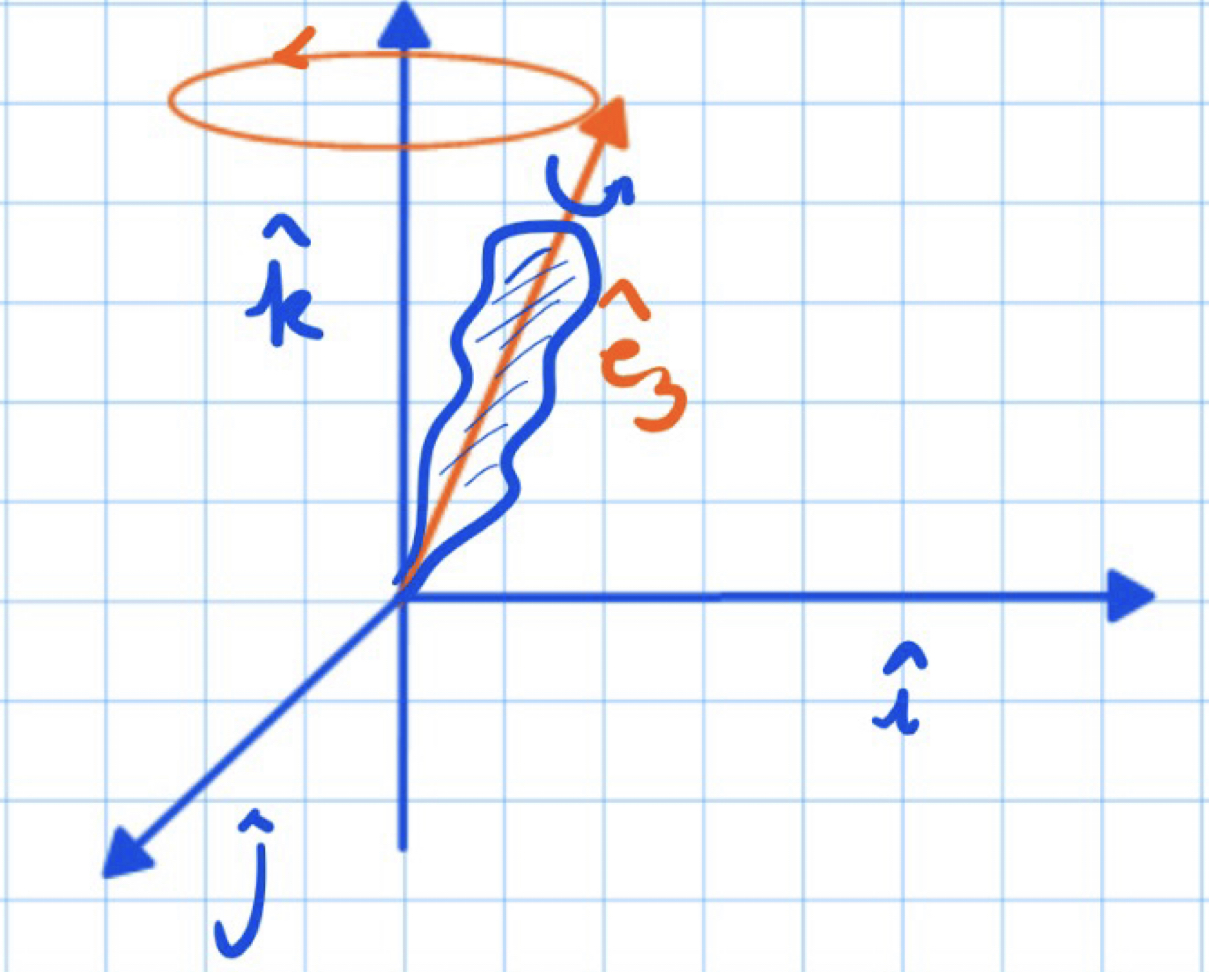
\includegraphics[width=0.17\textwidth]{Processionale.jpeg}
\end{wrapfigure}
%
\begin{defi}
Un moto di C è \textbf{Precessionale} se si possono scegliere $\theta \ e\ \theta'$ t.c. $\hat{e}_3\cdot\hat{k} = \ cost$\\
con $\hat{e}_3$ asse di rotazione propria e $\hat{k}$ asse di precessione
\end{defi}
Prop: Un moto di C è una precessione $\Longleftrightarrow \overline{\omega}= \lambda(t)\hat{k}+\mu(t)\hat{e}_3$ \ \ \ (+dim) \\
\phantom{}\\
\phantom{}\\
\phantom{}\\
\newpage


%
%Lezione 7
%
\subsection{Vincoli}
%
\begin{defi}
Un \textbf{vincolo} è una restrizione delle possibili configurazioni, moti e atti di un sistema di punti materiali.
\end{defi}
Un vincolo è della forma $F(\overline{x}_1, ..., \overline{x}_N, \overline{v}_1, ... , \overline{v}_N, t ) \geq 0$ \ \ dove $F:\mathbb{R}^{dN}\times\mathbb{R}^{dN}\times\mathbb{R}\rightarrow\mathbb{R} \ t.c \ \ \ F \in C^\infty(\mathbb{R}^{2dN}\times\mathbb{R})$\\
Oss: Ogni vincolo è uno scalare, noi quindi scriveremo un "vettore" di vincoli. \\ \\
%
%
%
I vincoli possono essere: \\
\ \ • \ \textbf{olonomo} se F non dipende dalle velocità \\
\ \ • \ \textbf{anolonomo} se F dipende dalle velocità \\
\ \ • \ \textbf{fisso} se F non dipende dal tempo\\
\ \ • \ \textbf{unilatero} se il vincolo è F(...) $\geq$ 0 \\
\ \ • \ \textbf{bilatero} se il vincolo è F(...) = 0 \\
Oss: Un vincolo anolonomo è integrabile se è equivalente a un vincolo olonomo \\
%
%
%
\begin{Ndefi}
Le \textbf{coordinate libere}, o lagrangiane, sono un insieme minimale di parametri sufficiente a caratterizzare univocamente un sistema di punti materiali, Il \textbf{grado di libertà} g è il numero di coordinate libere\\
Dati N punti materiali senza vincoli ottengo $g_0=dN$ gradi
\end{Ndefi}
%
%
%
Varietà delle configurazioni di un sistema vincolato (olonomi, bilateri) al tempo t è:

$\Sigma_t := \{ (\overline{x}_1, ..., \overline{x}_N) \in \mathbb{R}^{dN} \ t.c. \ \overrightarrow{F}(\overline{x}_1, ..., \overline{x}_N, t ) = 0 \}$ \\ \\
%
%
%
Dati M vincoli [ $\overrightarrow{F} = (F_1,...,F_M)$ ] olonomi e bilateri, si dicono:\\
\ \ • \ \textbf{compatibili} \ se $\Sigma_t \neq 0 \ \ \ \forall t \in \mathbb{R}$ \\
\ \ • \ \textbf{indipendenti}\ se $J_{ij}= \frac{\partial F_i}{\partial x_j} \implies rank(J_F)$ è massimo $\forall t \in \mathbb{R}$ \ \ \ \ allora $rank(J_F) = min \{ M,dN\} $ \\ \\
%
%
%
Teorema: Dato un sistema di $N\in\mathbb{N} \cup \{ +\infty \}$ punti materiali, sottoposto a M $\leq$ dN vincoli \\
\phantom{\ } Olonomi, bilateri, compatibili, indipendenti e fissato t, allora esistono: \\
\phantom{\ } $D_t$ (intorno di $\Sigma_t)\subset \mathbb{R}^{dN}$, \ \ un aperto $E_t\subset\mathbb{R}^g$ con g=dN-M, \\ 
\phantom{\ } Una funzione invertibile $\Phi : E_t \rightarrow D_t \ t.c. \ \ \Phi \in C^\infty(D_t)$ \ e \ $\overrightarrow{F}(\overrightarrow{\Phi}(\overline{q}),t) = \overline{0}$ \\
Oss: Questo teorema equivale alla generalizzazione a dN variabili del teorema della funzione implicita (Dini). \\ \\
%
%
%
Oss: Dato un sistema con $g_0$ gradi di libertà iniziali, dopo l'applicazione di M vincoli \\
\phantom{Oss: }Compatibili e indipendenti, avrò: \ \ \ \ \ \ \ \ $g=g_0-M$ \ (ovviamente se $g_0 \leq M$ avrò g=0) \\ \\
%
%
%Lezione 8
%
Dato un punto materiale P, $\overline{v}_P'$ è una sua \textbf{velocità virtuale} se $(\overline{x}_P,\overline{v}_P')$ è un atto di moto possibile per P.\\\
$\delta\overline{x}_P'$ è un suo \textbf{spostamento virtuale} se $\exists \delta t > 0 \ t.c. \ \delta\overline{x}_P' = \overline{v}_P'\delta t $\\
L'insieme delle velocità e spostamenti virtuali sono indicati con $V_P'(\overline{x}_P) \ e \ S_P'(\overline{x}_P)$ \ \ \ \ \ \ \ \ \ \ \
%
%
%
\begin{wrapfigure}{r}{0.32\textwidth}
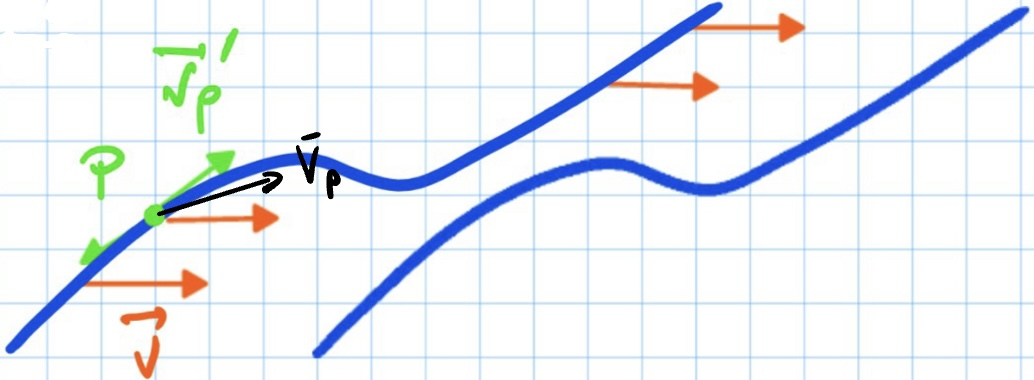
\includegraphics[width=0.32\textwidth]{Virtuali.jpeg}
\end{wrapfigure} \\
%
Oss: I valori virtuali dipendono dai vincoli.\\
Oss: A volte la velocità virtuale ha poco a che fare con quella reale \\
\phantom{Oss: }Per esempio quando il vincolo si muove ($\overline{v}$), abbiamo $\overline{v}_P = \overline{v}_P' + \overline{v}$  \ \\*
%
%
%
Le velocità virtuali sono \textbf{reversibili} se per ogni $\overline{v}_P'$ che è velocità virtuale, allora anche $-\overline{v}_P'$ lo è.

Vale lo stesso per gli spostamenti e gli spostamenti virtuali sono reversibili se e solo se lo sono le velocità.

Valori virtuali associati a vincoli bilateri sono sempre reversibili. \ \ \ \ \ \ \ \ \ \ \ \ \ \ \ \ \ \ \ \ \ \ \ \ \ \ \ \ \ \ \ \ \ \ \ 
%
%
%
%
\begin{wrapfigure}{l}{0.18\textwidth}
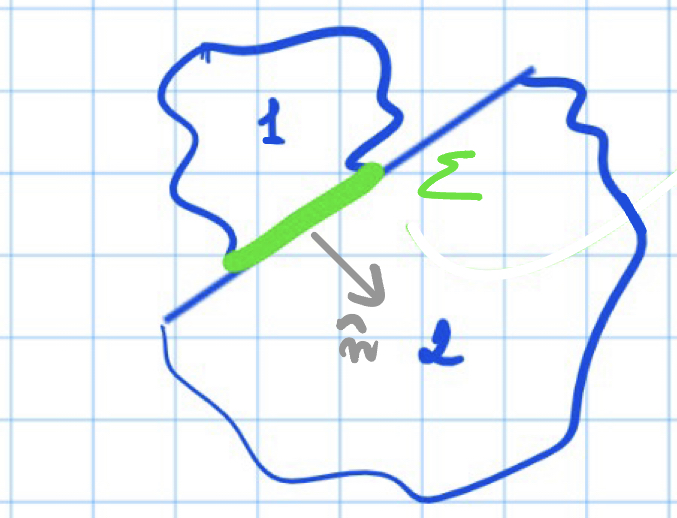
\includegraphics[width=0.18\textwidth]{Contatto.jpeg} \\ \\
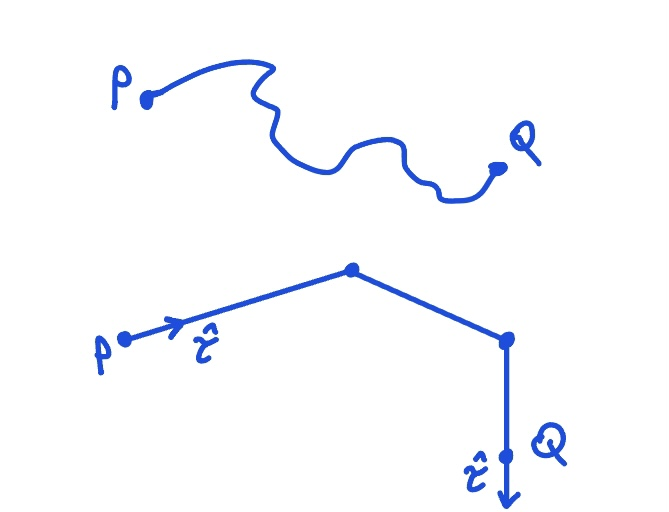
\includegraphics[width=0.18\textwidth]{Filo.jpeg}
\end{wrapfigure} \\
%
Vincoli anolonomi tra superfici $\Sigma$ \ \ (di contatto o di appoggio):\\
\textbf{contatto} \ (bilatero) \ \ \ $\overline{v}_{P_1}\cdot\hat{n} =\overline{v}_{P_2}\cdot\hat{n} \ \ \ \ \forall P \in \Sigma$ \\
\textbf{appoggio} (unilatero) \ $(\overline{v}_{P_1} -\overline{v}_{P_2})\cdot\hat{n} \leq 0 \ \ \forall P \in \Sigma$ \ (vincolo vale finché c'è contatto) \linebreak \\ \\
%
%
Vincoli olonomi su un Filo:\\
\textbf{inestensibile} (unilatero) $|\overline{PQ}| \leq l$\\
\textbf{in tensione} \ (bilatero) $\overline{V}_P\cdot \hat{\tau} = \overline{V}_Q\cdot\hat{\tau} \ \ \forall P,Q$ nel filo \\ \\
%
%
%
\textbf{Puro Rotolamento} è un vincolo anolonomo e\\
\ • \ \ unilatero se disco è appoggiato $\overline{v}_P  \cdot \hat{j} \geq 0 \ \ \forall t \in \mathbb{R} \ t.c. \ y_P(t)=0$\\
\ • \ \ bilatero se disco è vincolato a rotolare sulla guida, quindi \ \ $y_P(t)=0 \ \forall t \in \mathbb{R}$

Inoltre abbiamo il vincolo $\overline{v}_{P_{disco}}=\overline{v}_{P_{guida}}$ \ \ (anche se i punti di contatto cambiano) \\
Oss: Se la guida è fissa $\overline{v}_P=0$\\
Oss: Essendo un corpo piano $g_0=3$ e avendo i due vincoli (contatto e rotolalmento), otterremo g=1 \\
Oss: In ogni istante il punto P (di contatto) sarà il CIR e \ \  $\overline{x}_C(t)=\overline{x}_C(0) + R(\theta(t) - \theta(0))\hat{i}$ \\
Oss: In generale i vincoli di contatto possono essere di \textbf{strisciamento} se: $\overline{v}_{A_1} \cdot \hat{\tau} \neq \overline{v}_{A_2} \cdot \hat{\tau}$ \\
%
%
%
\begin{defi}
Un \textbf{sistema olonomo} è un sistema sottoposto a M vincoli bilateri, olonomi e fissi che assumeremo\\
Compatibili e indipendenti, allora avrà g = gradi di libertà = dN - M 
\end{defi}
%
%
%
Per ogni sistema olonomo esistono delle coordinate libere $\overline{q} \in \mathbb{R}^g$, per le quali ho un cambiamento di base

Regolare e invertibile t.c. $\overline{x}=X(\overline{q})$ e $\overline{q}=Q(\overline{x})=X^{-1}(\overline{x})$ \\ \\
%
%
%
%Date $\dot{q}_j$ e $\ddot{q}_j$ velocità e accelerazioni generalizzate, abbiamo $\overline{v}_i(t)=\sum_{j=1}^g\frac{\partial\overline{x}_i}{\partial q_j}\dot{q}_j \ \ \overline{a}_i(t)=\sum_{j,k=1}^g\{ \}$


\newpage

\section{Leggi della Dinamica}

Oss: A differenza della statica la dinamica dipenderà dalla scelta dell'osservatore
\subsection{Principi della Dinamica}
%
%
\begin{defi}
\textbf{I principio dinamica o principio d'Inerzia}\\
Esiste almeno un sistema (osservatore) di rifermento inerziale.
\end{defi}
Oppure: Esiste una classe non vuota di sistemi inerziali in moto rettilineo uniforme (stesse accelerazioni)\\
%
%
%
\begin{defi}
\textbf{II principio dinamica o legge di Newton}\\
Dato un punto materiale P e un osservatore inerziale, \ $\exists$ \ massa inerziale $m>0$, \ forza $\overline{F}\in\mathbb{R}^d$ \ t.c. \\
\phantom{} \hspace{2in} $m\overrightarrow{a}=\overrightarrow{F}$
\end{defi}
%
%
Oss: Legge di Newton è covariante, cioè è invariante per cambiamento di osservatore inerziale ($\overline{a}=\overline{a}'$)

Infatti sia R il cambio di base, allora $m\overline{\ddot{x}}=\overline{F} \Leftrightarrow mR\overline{\ddot{x}}'=R\overline{F}'$ \\ \\
%
%
%
Oss: La Forza è una grandezza fisica data, non è definita da legge Newton \\
Oss: $\overline{F}$ è un vettore applicato, serve definire il punto di applicazione \ \ $(\overline{F},P)$\\
Oss: Posso anche definire $\overline{F}=\overline{F}(\overline{x},\dot{\overline{x}},t)$ con $\overline{F}:\mathbb{R}^d\times\mathbb{R}^d\times\mathbb{R}\rightarrow\mathbb{R}^d$ t.c. $(\overline{F} \in C^\infty)$

Questo equivale a un pb. di Cauchy di d equazioni differenziali del 2° ordine: \ \ \ \
$\begin{cases}
\ddot{\overline{x}}=\dfrac{1}{m}\overline{F}( \overline{x},\dot{\overline{x}},t) \\
\dot{\overline{x}}(0) =\overline{v}_{0}\\
\overline{x}(0) =\overline{x}_{0}
\end{cases}$ \\
Condizione di esistenza e unicità: $\overline{F}$ \ Lipschitz su $A\subset\mathbb{R}^{2d}$ (aperto, limitato) e continua in T (posto $t\in[0,T)$)\\
Oss: Condizione necessaria affinché $\overline{f}$ sia Lipshitziana in A aperto è che esistano finite tutte le derivate parziali \\ \\
%
%
%
Oss: In un sistema di riferimento non inerziale la forza $\overline{F}'$ segue dal II principio e teorema di Coriolis: \\
\phantom{} \hspace{0.5in}  $m\overline{a}'=\overline{F} - m\{\dot{\overline{\omega}}\wedge\overline{x}'  +  \overline{\omega}\wedge(\overline{\omega}\wedge\overline{x}')  +  2\overline{\omega}\wedge\dot{\overline{x}}'\}$ \ \ \ (ovvero F reale - forze apparenti) \\
%
%
%
\begin{defi}
\textbf{III principio dinamica}\\
L'iterazione tra due punti materiali è data da due forze uguali e contrarie dirette lungo la congiungente:\\
\phantom{} \hspace{2in} $\overline{F}_1=-\overline{F}_2=f\frac{\overline{P_1P_2}}{|P_1P_2|}$\\
Una \textbf{coppia di forze} è data da due forze con stessa intensità, applicate a punti diversi: $(\overline{f},P) \ e \ (-\overline{f},P')$
\end{defi}



%Lezione10

\subsection{Forze}
%
Tipi di Forze $\overline{F}(\overline{x}, \dot{\overline{x}},t)$:\\
\ • \ \ \textbf{interna} se dovuta dall'interazione con altri punti del sistema (III principio)\\
\ • \ \ \textbf{esterna} altrimenti \\
\ • \ \ \textbf{costante} se $\overline{F} = \overline{F}_0 \in \mathbb{R}^d$\\
\ • \ \ \textbf{posizionale} se $\overline{F} = \overline{F}(\overline{x})$\\
\ • \ \ \textbf{centrale} se è posizionale ed $\exists O \in \mathcal{E}_d$ (centro) \ t.c. $\overline{F}(\overline{x})=f(|\overline{x}-\overline{x}_0|)\cdot \frac{\overline{x}-\overline{x}_0}{|\overline{x}-\overline{x}_0|}$\\
%
%
%
\begin{defi}
Data una forza posizionale $\overline{F}(\overline{x})$ e una curva $\Gamma$ parametrizzata da $\overline{\gamma}:[s_0,s_1]\rightarrow\mathbb{R}^d$\\
Il \textbf{lavoro} compiuto da $\overline{F}$ lungo $\Gamma$ è \ \ \ $L=\int^{s_1}_{s_0} \overline{F}(\overline{\gamma}(s))\cdot\overline{\gamma}'(s)ds$
\end{defi}
%
%
%
Oss: Il lavoro infinitesimo di $\overline{F}$ in $d\overline{x}$ è $dL = F_1dx_1 + F_2dx_2+ F_3dx_3$ cioè una 1-forma differenziale\\
%
Una 1-forma differenziale è $\omega=\sum_{j=1}^3 f_j(\overline{x})dx_j$ e in A aperto di $\mathbb{R}^3$ è:\\
\ • \ \ \textbf{esatta}  se $\exists g:A\rightarrow\mathbb{R}^3, g\in C^1(A) \ t.c. \ \ \omega = dg = \sum_{j=1}^3 \frac{\partial g}{\partial x_j} \ dx_j$ \\
\ • \ \ \textbf{chiusa} se $d\omega=0$ dove $d\omega= \sum_{j=1}^3 \partial F_j \wedge dx_j$ \\
%
Oss: La forma differenziale del lavoro in un dominio semplicemente connesso A è esatta  $\ \Leftrightarrow \ \frac{\partial F_i}{\partial x_j}=\frac{\partial F_j}{\partial x_i} \ \ \forall \overline{x}\in A$\\
%
Oss: Se dL è esatta e $\overline{F}\in C^1(A) \implies \frac{\partial F_i}{\partial x_j}=\frac{\partial F_j}{\partial x_i}$ in A \\ \\
%
%
%
Teo: Ogni forma $\omega$ esatta è anche chiusa, ovvero $d^2\omega = 0$\\
Teo: In un aperto semplicemente connesso di $\mathbb{R}^n$ ogni 1-forma differenziale chiusa è anche esatta\\ 
%
Prop: Se la forma dL è esatta $\implies \int_{\Gamma_0} dL = 0 \ \ \ \forall \ \Gamma_0$ curva chiusa \ \ \ (+dim)\\ 
%
Teo: Condizione necessaria affinché dL sia esatta è che $\overline{F}$ sia posizionale\ \ \ (+dim)\\
%
%
%
\begin{defi}
$\overline{F}$ posizionale è \textbf{conservativa} in $A\subset\mathbb{R}^3$ \ \ se $\exists$ \textbf{potenziale} $U\in C^2(A) \ t.c. \ \ \overline{F}(\overline{x})=-\nabla U(\overline{x})$
\end{defi}
%
Teo: In A aperto semplicemente connesso di $\mathbb{R}^3 \ \ \ \overline{F}$ posizionale e conservativa $\Leftrightarrow \ \nabla \wedge \overline{F} = \overline{0}$ \ \ \ (+dim)\\
\phantom{} \hspace{0.23in} dove $(\nabla\wedge\overline{F})_i = \sum^3_{j,k=1} \varepsilon_{ijk} \frac{\partial}{\partial x_j}F_k$ \\ \\
%
%
%
Una forza $\overline{F}$ si dice \textbf{attiva} se è nota a priori la sua dipendenza da $\overline{x}, \dot{\overline{x}}$ e t\ \ cioè $\overline{F}=\overline{F}(\overline{x},\dot{\overline{x}},t)$ \\
In ogni altro caso di dice \textbf{reazione vincolare} $\overline{\Phi}$ \ ed è dovuta dalla presenza di un vincolo\\
%
Oss: La legge di Newton si può riscrivere: \ \ $m\overline{a} = \overline{F}^{(att)} + \overline{\Phi}$ \\ \\
%
% 
%
Esempi di forze e potenziali:\\
\ • \ \ Forza \textbf{peso} è una forza costante, $\overline{F}_g=m\overline{g}$ \ con $\overline{g}=-g\hat{j}$\\
\phantom{} \hspace{0.18in} Le forze costanti sono conservative con $U(\overline{x})=-\overline{F}_0\cdot\overline{x}$ \hspace{0.18in} per $\overline{F}_g: \ \ U_g(\overline{x})= mgy$\\
%
\ • \ \ Forza \textbf{elastica} è una forza posizionale, $\overline{F}_{el}(\overline{x})=-k(\overline{x}-l)\hat{x}$ \hspace{0.18in} $U_{el}(\overline{x})=\frac{1}{2}k(|\overline{x}|-l)^2$\\
%
\ • \ \ Forza \textbf{gravitazionale} è una forza posizionale, $\overline{F}_{1,2} = -G\frac{m_1m_2}{r^2}\hat{r} \ \ \ (\overline{r}=\overline{x}_1 - \overline{x}_2$)\\
\phantom{} \hspace{0.18in} Se $m_2=M>>m=m_1$ allora diventa una forza centrale in $\overline{x}_2$ \ \ e avremo $f(\overline{r}) = \overline{F}_{1,2}(\overline{x}_1 , \overline{x}_2)$\\
\phantom{} \hspace{0.18in} Le forze centrali sono conservative con $U(\overline{r})=g(|\overline{r}|)$ dove g è la primitiva di $-f(\overline{r})$ \hspace{0.12in} $U_G(\overline{r})= -\frac{GMm}{r}$\\

\newpage




\section{Statica}
%
%
%
\subsection{Equazioni Cardinali della Statica}
%
\begin{defi}
Le equazioni del moto $\overline{F}=m\overline{a}$ per un punto materiale ammettono\\ una \textbf{soluzione di quiete} in $\overline{x}_0\in\mathbb{R}^d$\ \
se $\overline{x}(t)=\overline{x}_0, \forall t \in \mathbb{R}$ è soluzione delle eq. stesse
\end{defi}
%
\begin{defi}
Un sistema di N punti materiali sottoposto alle forze $\{\overline{F}_j(\overline{x}_1,...,\overline{x}_N,\overline{v}_1,...,\overline{v}_N,t)\}$\\
Ha una \textbf{configurazione di equilibrio} $\{\overline{x}_{j\in\{1...N\}}^{(0)}\}$ \ \ \ se \
$\overline{F}_j(\overline{x}_1^{(0)},...,\overline{x}_N^{(0)},\overline{0},...,\overline{0},t)=\overline{0} \ \ \forall t,j$
\end{defi}
%
Oss: Se la forza è Lipschitz, $\{\overline{x}_{j\in\{1...N\}}^{(0)}\}$ è soluzione di quiete se e solo se è configurazione di equilibrio \\
Oss: Le forze si possono sempre scomporre: \ \
$\overline{F}_j=\overline{F}_j^{(ext)}+\overline{F}_j^{(int)}=\overline{F}_j^{(att)}+\overline{\Phi}_j$ \\
%
%
%
\begin{defi}
Data una forza $(\overline{f},\overline{x}_P)$ applicata in P, il suo \textbf{momento} rispetto al \textbf{polo} O è $\overline{m}=(\overline{x}_P-\overline{x}_O)\wedge\overline{f}$
\end{defi}
Oss: Avremo $|\overline{m}|= |\overline{OP}||\overline{f}||sen\theta|$ \ e \ $\overline{m}=m \ \hat{k}$\\ \\
%
Un \textbf{sistema di forze} \ $\mathcal{S}=\{(\overline{f}_1,\overline{x}_1),...,(\overline{f}_n,\overline{x}_n)\}$ è una collezione di vettori applicati
\begin{Ndefi}
La \textbf{risultante} e il Momento risultante di $\mathcal{S}$ rispetto a O sono: \ \ $\overline{R}=\sum_{j=1}^n\overline{f}_n \ \ \ \overline{M}_O=\sum^n_{j=1}(\overline{x}_j-\overline{x}_0)\wedge\overline{f}_j$
\end{Ndefi}
%
%Lezione11
%
Teorema: Condizione necessaria per un sistema meccanico in configurazione di equilibrio è che il sistema \\ \phantom{\ } di forze esterne rispetti le \textbf{equazioni cardinali della statica:} $\ \ \overline{R}^{(ext)}=\overline{0}, \ \ \overline{M}_O^{(ext)}=\overline{0} \ \ \forall O \in \mathcal{E}_3$ \ \ \ (+dim)\\
%
Lemma: Per ogni sistema meccanico il sistema di forze interne ha: $\ \ \overline{R}^{(int)}=\overline{0}, \ \ \overline{M}_O^{(int)}=\overline{0} \ \ \forall O \in \mathcal{E}_3$ \ \ \ (+dim)\\ \\
%
%
%
Oss: Dato un sistema in una conf di eq, le equazioni cardinali valgono anche per i suoi sottosistemi\\
%
Prop: Trasporto del momento \ \ \ (+dim)\\
\phantom{Prop: }Dato un sistema di forze $\mathcal{S}$ e due poli O, O' $\in \mathcal{E}_d$ si ha: $\overline{M}_{O'}=\overline{M}_O + \overline{OO'}\wedge\overline{R}$





\subsection{Sistemi di Forze}
%
\begin{defi}
Due sistemi di forze $\mathcal{S}, \mathcal{S}'$ si dicono \textbf{equivalenti} $\mathcal{S} \sim \mathcal{S}'$ \ se $\overline{R}=\overline{R}' \ e \ \overline{M}_O=\overline{M}_O' \ \forall O \in \mathcal{E}_3$
\end{defi}
%
%
Oss: L'equivalenza tra sistemi di forze è una relazione di equivalenza, cioè valgono le proprietà:\\
\phantom{Oss: }i) riflessiva: $\mathcal{S} \sim \mathcal{S}$ \ \ \ ii) simmetrica: $\mathcal{S} \sim \mathcal{S}' \Leftrightarrow \mathcal{S}' \sim \mathcal{S}$ \ \ \ iii) transitiva: $\mathcal{S} \sim \mathcal{S}' \ e \ \mathcal{S}' \sim \mathcal{S}'' \implies \mathcal{S} \sim \mathcal{S}''$ \\
%
%
%
\begin{defi}
L'\textbf{invariante scalare} di $\mathcal{S}$ rispetto a O è \ $I=\overline{R}\cdot\overline{M}_O$ \ \ \ I non dipende dal polo scelto
\end{defi}
%
%
Prop: Dato $\mathcal{S}$ con $\overline{R}\neq \overline{0}, \ \exists h$ retta dell'\textbf{asse centrale} t.c. \ $\overline{M}_P /\!\!/ \overline{R} \ \ \forall P\in h$ \ \ e $h: \overline{x}=\lambda\overline{R}+\frac{\overline{R}\wedge\overline{M}_A}{|\overline{R}|^2} + \overline{x}_A$\\
\phantom{Prop: }con $A\in \mathcal{E}_3$ qualsiasi \phantom{\ \ \ } E se I=0, h è detto asse di applicazione della risultante e $\overline{M}_P=\overline{0}$ \ \ \ (+dim)\\ \\
%
%
%
Prop: Ogni sistema di forze è equivalente al più a una forza più una coppia di forze. \ \ \ (+dim)\\
%
Teo: Dato un sistema di forze $\mathcal{S}$ si ha uno dei seguenti casi: \ \ \ (+dim)\\
\phantom{\ \ \ \ \ \ } i) $\overline{R}=\overline{0}, \ \overline{M}_O=\overline{0} \Leftrightarrow \mathcal{S}\sim\emptyset$ \hspace{0.77in}
ii) $\overline{R}=\overline{0}, \ \overline{M}_O\neq\overline{0} \Leftrightarrow \mathcal{S}\sim$ coppia di forze \\
\phantom{\ \ \ \ \ \ } iii) $\overline{R}\neq\overline{0}, \ I=\overline{0} \Leftrightarrow \mathcal{S}\sim\{(\overline{R},P)\}, P\in h$ \ \ \ \ \
iv) $\overline{R}\neq\overline{0}, \ I\neq\overline{0} \Leftrightarrow \mathcal{S}\sim\{(\overline{R},O),(\overline{f},O),(-\overline{f},P)\}$ \\
%
Lemma: Siano $\mathcal{S}, \mathcal{S}'$ t.c. $\overline{R}=\overline{R}' \ e \ \overline{M}_O=\overline{M}_O'$ per un centro $O \in \mathcal{E}_3 \Leftrightarrow \mathcal{S} \sim \mathcal{S}'$ \ \ \ (+dim)\\
%Oss: Per verificare l'equivalenza è sufficiente $\overline{R}=\overline{R}' \ e \ \overline{M}_O=\overline{M}_O'$ per un singolo O (trasporto del momento) \\ \\
%
%
%
\begin{defi}
Il \textbf{centro di massa} è per un sistema discreto $\overline{x}_{cm}=\frac{1}M \sum_{j=1}^Nm_j\overline{x}_j$\ dove $M=\sum_{j=1}^Nm_j$\\
%
Per un sistema continuo $\exists \rho :\mathbb{R}^3\rightarrow\mathbb{R}^+$ detta distribuzione di massa t.c. \ $m_A=\int_A\rho(\overline{x})d\overline{x}$ è la massa in A\\
\phantom{\ \ \ \ } Allora la massa totale diventa \  $M=\int_{\mathbb{R}^3}\rho(\overline{x})d\overline{x}$ \ \ e \ \ $\overline{x}_{cm}=\frac{1}M \int_{\mathbb{R}^3} \overline{x}\rho(\overline{x})d\overline{x}$
\end{defi}
%
%
Oss: La forza peso applicata a un sistema è equivalente alla forza $\overline{F}_P=M\overline{g}$ applicata nel centro di massa
%
%Lezione 12
%
\subsection{Vincoli Ideali}
%
Dato un punto materiale con velocità $\overline{v}$, la \textbf{potenza istantanea} generata dalle forze $\overline{F}$ è $\Pi=\overline{F}(\overline{x},\overline{v},t)\cdot \overline{v}$ \\
%
Dato un moto $\overline{\gamma}(t):\mathbb{R}\rightarrow\mathbb{R}^3$ di un punto soggetto a $\overline{F}(\overline{x},\overline{v},t)$, allora il lavoro è:\\
\phantom{}\hspace{2in} $L \ =\ \int^{t_1}_{t_0} \dot{\overline{\gamma}}(\tau)\cdot\overline{F}(\overline{\gamma}(\tau),\dot{\overline{\gamma}}(\tau),\tau)\ d\tau \ = \ \int\Pi(\tau)d\tau$ \\
%
%
%
\begin{defi}
Dato un sistema di punti $P_j$ sottoposti alle forze $\overline{F}_j$, il \textbf{lavoro} e la \textbf{potenza virtuali} sono:\\
\phantom{\ \ \ } $\delta L'=\sum^N_{j=1}\overline{F}_j\cdot\delta x_j' \ con \ \delta x_j' \in S_j' \ \ \forall j \in \{ 1...N\}$
\ \ \ \ $\Pi'=\sum^N_{j=1}\overline{F}_j\cdot v_j' \ con \ v_j' \in V_j' \ \ \forall j$
\end{defi}
%
%
%
\begin{defi}
I vincoli a cui è sottoposto un sistema di punti sono \textbf{ideali} se generano solo reazioni vincolari \\
$\{\overline{\Phi}_j\}_{j\in\{1...N\}}$ che producono lavoro virtuale o potenza virtuale non negative \\
Ovvero \ \ \ $\sum^N_{j=1}\overline{\Phi}_j\cdot\delta x_j'\geq 0 \ \ \forall \delta x_j' \in S_j' \ \forall j$ \ \ oppure se \ \ \ $\sum^N_{j=1}\overline{\Phi}_j\cdot v_j'\geq 0 \ \ \forall v_j' \in V_j' \ \forall j$
\end{defi}
Oss: Un vicolo \textbf{perfetto} è un vincolo ideale e bilatero \ \ (al posto del $\geq$ c'è =)\\
\phantom{Oss: }Un vicolo è liscio se non produce attrito e quindi la reazione vincolare è $\perp$ alla superficie di contatto \\
Oss: Tutti i vincoli che useremo sono ideali: incastro, cerniera, manicotto, carrello, \\
\phantom{Oss: }puro rotolamento, filo in tensione, guida e appoggio in assenza di attrito \\
%
%
%
%\subsection{Principio dei lavori virtuali}
%
\begin{defi}
Un'\textbf{equazione pura} caratterizza statica e dinamica di un sistema e non contiene reazioni vincolari
\end{defi}
%
%
%
Teorema: Principio dei lavori virtuali, o PLV \ \ \ (+dim)\\
\phantom{\ } Dato un sistema di punti sottoposto a vincoli ideali e \underline{fissi} la configurazione $\{P-j^{(0)}\}_{j\in\{1...N\}}$ è di equilibrio\\ \phantom{\ \ } se e solo se \ $\delta L'^{(att)}=\sum^N_{j=1}\overline{F}_j^{(att)}\cdot \delta \overline{x}_j'\leq 0 \ \ \  \forall\delta\overline{x}_j'\in S_j' \ \ \ \forall j$ \ \ \ (per vincoli perfetti c'è = invece di $\leq$)

\newpage
%Lezione13

\subsection{Statica dei Sistemi Olonomi}
%
Siano: g= $\#$g.d.l. \ \ $\overline{q}$= coordinate libere \ \ $\overline{X}(\overline{q})$ fornisce coordinate originali in funzione di quelle libere.

Gli spostamenti virtuali  $ \delta \overline{x}_j' = \sum_{i=1}^g \frac{\partial \overline{x}_j}{\partial q_i}\cdot \delta q_i'$ \ \ (analogo per velocità virtuali)\\ \\
%
%
%
Prop: Lavoro virtuale delle forze attive per sistema olonomo è \ $\delta L'^{(att)}=\sum_{k=1}^gQ_k\delta q_k'$ \\ 
\phantom{Prop: }Dove $Q_K$ sono le componenti generalizzate delle forze attive \ \ $Q_k = \sum_{j=1}^N\overline{F}_j^{(att)}\frac{\partial\overline{x}_j}{\partial q_k}$ \ \ \ (+dim) \\
%
%
%
Prop: Un sistema olonomo è in equilibrio in $\overline{q}^{(0)} \ \Leftrightarrow \ Q_k(\overline{q}^{(0)})=0 \ \ \forall k \in \{1...g\}$ \ \ \ (+dim) \\ \\
%
%
%
Oss: Se le forze attive sono conservative, cioè $\exists \widetilde{U}:\mathbb{R}^{dN}\rightarrow\mathbb{R} \ t.c. \ \overline{F}_j^{(att)}=-\nabla_j\widetilde{U}(\overline{x}_1,...,\overline{x}_N)$, \\
\phantom{Oss: }Si definisce il potenziale in funzione delle coordinate generalizzate \ \ $U(\overline{q})=\widetilde{U}(\overline{x}_1(\overline{q}),...,\overline{x}_N(\overline{q}))$ \\
Teo: Sistema olonomo con forze attive conservative è in equilibrio in $\overline{q}(0) \ \Leftrightarrow \ \frac{\partial U}{\partial q_k}(\overline{q}^{(0)})=0 \ \ \forall k$ \ \ \ (+dim)\\
%
%
%
\begin{defi}
Per un sistema olonomo avremo \textbf{configurazioni ordinarie} se $\overline{q} \in \Sigma^0$ (parte interna) \\
\textbf{Di confine} se $\overline{q} \in \partial\Sigma$ dove $\Sigma$ è lo spazio delle soluzioni ammissibili \ \ (serve per vincoli unilateri)
\end{defi}
%
Oss: Lo spazio degli spostamenti virtuali cambia in base al tipo di configurazione: \ \ $S'(\overline{q}) = \begin{cases}\mathbb{R}^g \ se \ \overline{q} \in \Sigma^0 \\ \neq\mathbb{R}^g \ se \ \overline{q} \in \partial\Sigma \end{cases} $ \\
%
Prop: Una configurazione $\overline{q}^{(0)}$ ordinaria è di equilibrio \ $\Leftrightarrow \ Q_k(\overline{q}^{(0)})=0 \ \forall k$ \\
\phantom{Prop: }Una $\overline{q}^{(0)}$ è di confine allora $\exists \tilde{k} \in \{1...g\} \ t.c. \ \delta q_{\tilde{k}}'\geq 0$ oppure $\delta q_{\tilde{k}}'\leq 0$ \\
\phantom{Prop: }Inoltre $\overline{q}^{(0)}$ è di equilibrio $\Leftrightarrow \begin{cases}
Q_k(\overline{q}^{(0)})=0 \ \forall k \ t.c. \ \delta q_k' \in \mathbb{R} \\
Q_k(\overline{q}^{(0)})\geq 0 \ \forall k \ t.c. \ \delta q_k' \leq 0 \\
Q_k(\overline{q}^{(0)})\leq 0 \ \forall k \ t.c. \ \delta q_k' \geq 0
\end{cases}$ 



\subsection{Statica del Corpo Rigido}
%
Prop: Un copro rigido sottoposto a $\mathcal{S}^{(ext)}$, vale: \  $\delta L' = \overline{R}^{(ext)}\cdot\delta\overline{x}_C' + \overline{M}_C^{(ext)}\cdot\overline{\varepsilon} $ \ \ con $\overline{\varepsilon}=\overline{\omega}\delta t \in \mathbb{R}^3$ \ \ \ (+dim)\\
Prop: Per un corpo rigido con vincoli ideali e fissi \ \ equazioni cardinali $\Leftrightarrow$ configurazioni di equilibrio \ \ \ (+dim)\\
%
%
%
\begin{defi}
Il \textbf{Poligono di appoggio} di un corpo rigido appoggiato su un piano $\Pi$ in un numero finito di punti è l'unico poligono t.c. \ \ \ i) ogni vertice è un punto d'appoggio (non viceversa) \ ii) il poligono è convesso  \\
\phantom{} \hspace{1.4in} iii) i punti di appoggio che non sono vertici, non sono esterni al poligono
\end{defi}
%
Prop: Un corpo rigido appoggiato è in equilibrio \ $\Leftrightarrow$ \ la proiezione di G su $\Pi$ è dentro al poligono \ \ \ (+dim)\\

\newpage





%
%Lezione14
%

\section{Dinamica}

\subsection{Quantità Meccaniche}
%
\begin{Ndefi}
Dato un punto materiale di massa m>0, le sue quantità meccaniche sono: \\
\ • \ \textbf{quantità di moto}, o impulso, \ $\overline{Q}=m\overline{v}$ \hspace{1.05in} • \ \textbf{energia cinetica} \ $T=\frac{1}{2}m|\overline{v}|^2$ \\
\ • \ \textbf{momento angolare} rispetto al polo O \ $\overline{K}_O = \overline{OP}\wedge\overline{Q}$ \ \ \ \ \ \ • \ \textbf{potenza} \ $\Pi = \overline{F}\cdot\overline{v}$
\end{Ndefi}
%
Oss: Le quantità meccaniche dipendono dall'osservatore e sono estensive (somma dei sottosistemi)\\ \\
%
%
%
Prop: Legge trasporto momento angolare \ \ \ $\overline{K}_{O'}=\overline{K}_O + \overline{O'O}\wedge\overline{Q}$ \ \ (+dim) \\
%
Prop: L'impulso complessivo di un sistema è \ $\overline{Q}= M \overline{v}_G$ \ \ (con G= baricentro) \ \ (+dim)\\
%
Prop: Sia O' un osservatore solidale al centro di massa G di un sistema, allora \ \ $\overline{Q'}=\overline{0}$ \ \ (+dim)\\ \\
%
%
%
Teo: (K$\ddot{\text{o}}$nig 1) Per ogni sistema di punti materiali \ \ $T=\frac{1}{2} M |\overline{v}_G|^2 + \frac{1}{2} \sum_{j=1}^N m_j |\overline{v}_j'|^2$ \ \ (+dim)\\
Oss: In entrambi i teoremi $\overline{v}_j'$ sono le velocità relative a $\theta'$ solidale a G e in moto traslatorio rispetto a $\theta$ \\
%
Teo: (K$\ddot{\text{o}}$nig 2) \ \ \ (+dim)\\
\phantom{\ } Per ogni sistema $\overline{K}_O =\overline{K}'_G + M \ \overline{OG}\wedge\overline{v}_G$  \ \ dove $\overline{K}_G' = \sum^N_{j=1} m_j \overline{CP}_j \wedge \overline{v}_j'$ è indipendente dal polo scelto C





\subsection{Quantità Meccaniche per il Corpo Rigido}
%
\begin{defi}
Il \textbf{Momento inerzia} di un corpo rigido rispetto a un asse \ $r: \lambda \hat{u} + \overline{x}_Q$ è:
\ $I_r=\begin{cases}
\sum_{j=1}^N m_j dist^2(P_j;r) \ \ \text{discreto} \\
\int_{\mathbb{R}^d} d\overline{x} \rho (\overline{x}) dist^2(P;r) \ \ \text{continuo}
\end{cases}$
\end{defi}
%
Oss: La distanza punto-retta è data da: \ \ $dist(P;r) = |\overline{QP}\wedge\hat{u}|$ \\ \\
%
%
%
Teo: (Huygens-Steiner)  \ \ \ (+dim) \\
\phantom{\ }Dato un asse \ $r: \lambda \hat{u} + \overline{x}_Q$, \ \ $I_r=I_{r_G} + M dist^2(G;r) $ \ \ dove $r_G$ è l'asse $/\!/$ r passante per il centro di massa G \\
%
%
%
\begin{defi}
Il \textbf{Tensore di inerzia} di un sistema meccanico rispetto a O è la matrice simmetrica $\mathbb{I} \in M_3^{sym}(\mathbb{R})$ \\ \phantom{DEF: } data da: \ \ $\mathbb{I}_{lk}^{(O)}=
\begin{cases}
\sum_{j=1}^N m_j\{|\overline{OP}_j|^2 \delta_{lk} - (\overline{OP}_j)_l(\overline{OP}_j)_k\}\\
\int_{\mathbb{R}^3} \rho(\overline{x}) \{|\overline{x}-\overline{x}_O|^2 \delta_{lk} - (\overline{x}-\overline{x}_O)_l(\overline{x}-\overline{x}_O)_k\}d\overline{x}
\end{cases}$
\ \ con $k,l \in \{1,2,3\}$
\end{defi}
%
%
Prop: Dato un asse $\ \ r: \overline{x}=\lambda\hat{u}+\overline{x}_Q$ si ha \ \ $I_r = \hat{u}\mathbb{I}^{(Q)}\hat{u} = \sum_{l,k=1}^3\hat{u}_l\mathbb{I}^{(Q)}_{lk}\hat{u}_k$ \ \ \ (+dim) \\
%
%
%
\begin{defi}
$\mathbb{I}^{(O)}$ simmetrica e quindi diagonalizzabile con una matrice ortogonale O t.c. $O\mathbb{I}^{(O)}O^T=diag(I_1,I_2,I_3)$\\
%
Gli autovalori di $\mathbb{I}^{(O)}, \text{ cioè } I_1,I_2,I_3 \in \mathbb{R}^+$ sono detti \textbf{momenti principali di inerzia}\\
I relativi autovettori sono i vettori direttori di 3 assi passanti per O detti \textbf{assi principali di inerzia}
\end{defi}
%
%Lezione15
%
Prop: $\forall \overline{u}\in\mathbb{R}^3, \ \ \mathbb{I}^{(O)}\overline{u}=\begin{cases}
\sum_{j=1}^N m_j\overline{OP}_j \wedge (\overline{u}\wedge\overline{OP}_j)\\
\int_{\mathbb{R}^3}\rho(\overline{x})(\overline{x} - \overline{x}_O)\wedge[\overline{u}\wedge(\overline{x}-\overline{x}_O)]d\overline{x}\end{cases}$ \ \ \ (+dim)\\ \\
%
%
Prop: Il momento angolare di C rispetto a un polo $O\in\mathcal{E}_3$ soddisfa: $\ \overline{K}_O=\begin{cases} M\overline{OG}\wedge\overline{v}_G +\mathbb{I}^{(G)}\overline{\omega} \\ M\overline{OG}\wedge\overline{v}_O +\mathbb{I}^{(O)}\overline{\omega} \end{cases}$(+dim) \\
Oss: Il momento angolare si può scomporre in quello di G più quello di relativo a G \\
Oss: Se O è G o un punto fisso (anche CIR), allora \ $\overline{K}_O=\mathbb{I}^{(O)}\overline{\omega}$ \\ \\
%
%
%
Prop: Energia cinetica di corpo rigido C : \ \ $T=\frac{1}{2}M|\overline{v}_G|^2 + \frac{1}{2}\overline{\omega}\mathbb{I}^{(G)}\overline{\omega}$ \ \ \ (+dim)\\
Oss: Se ho un moto piano, allora $T=\frac{1}{2}I_r\omega^2(t)$ \ con $r: \overline{x}=\lambda\hat{k}+\overline{x}_{cir}$
%
%
%
\begin{defi}
L'\textbf{ellissoide di inerzia} associato a un corpo rigido è il luogo geometrico \ $\mathcal{E}:=\{\overline{\omega} \in \mathbb{R}^3 |\ \ \overline{\omega}\mathbb{I}^{(O)}\overline{\omega} =1\}$
\end{defi}
%
Oss: Gli assi dell'ellissoide sono gli assi principali di inerzia e vale \ $\mathcal{E}:=\{\overline{\omega} \in \mathbb{R}^3 |\ \ I_1\omega_1^2 + I_2\omega_2^2 + I_3\omega_3^2 =1\}$, \\
\phantom{Oss: }Quindi i semiassi sono lunghi $\frac{1}{\sqrt{I_j}}$.\\
%
Oss: Se $I_1<I_2<I_3$ allora i tre assi sono univocamente determinati e perpendicolari\\
%
Oss: Se due semiassi sono uguali, allora l'ellissoide è invariante per rotazione rispetto al terzo asse $\hat{e}_3$\\
\phantom{Oss: }e qualsiasi asse $\perp \hat{e}_3$ è di inerzia, l'ellissoide si dirà di rotazione e il corpo associato giroscopio\\
Oss: Viceversa se due assi di inerzia non sono ortogonali, i rispettivi momenti coincidono\\
%
%
%
\begin{defi}
Un C ha un \textbf{asse di simmetria} di ordine n $\ge$ 2 se C si sovrappone a se stesso dopo \\ 
\phantom{DEF. } una rotazione di $\frac{2\pi}{n}$ attorno a tale asse, inoltre se $n\in\mathbb{N}_0$ si dirà asse di simmetria rotazionale
\end{defi}
%
Oss: Asse sim per C di ordine n $\implies$ asse sim per $\mathcal{E}$ di ordine $\ge$ n \\ \\
%
%
%
\ • \ \ r asse principale di inerzia $\Leftrightarrow$ r asse sim ordine $\ge$ 2 per $\mathcal{E}$ \\
\ • \ \ asse sim ordine > 2 per $\mathcal{E}$ è asse sim rotazionale \\
\ • \ \ 2 assi sim ordine 2 per $\mathcal{E}$ con angolo $\neq \frac{\pi}{2} \implies \mathcal{E}$ è ellissoide di rotazione \\
\ • \ \ 2 assi sim ordine > 2 per $\mathcal{E} \implies \mathcal{E}$ è una sfera \\
\ • \ \ 2 assi sim, uno con ordine > 2 e angolo $\neq \frac{\pi}{2} \implies \mathcal{E}$ è una sfera \\
%
%
%
\ • \ \ C ha un asse di simmetria di ordine $\ge 2 \implies$ è un asse principale di inerzia \\
\ • \ \ C ha 2 assi di simmetria di ordine > 2 $\implies \mathcal{E}$ è una sfera e $I_1=I_2=I_3$ \\
\ • \ \ C ha 2 assi di simmetria uno con ordine > 2 e angolo $\neq \frac{\pi}{2} \implies  \mathcal{E}$ è una sfera e $I_1=I_2=I_3$ \\ \\
%
%
%
Prop: Se C ha un asse di simmetria r allora $G \in r$, se ne ha due G è all'intersezione dei due


\subsection{Equazioni Cardinali della Dinamica}
%
Teo: Lungo qualunque moto di un sistema di punti sono verificate le \textbf{equazioni cardinali della dinamica}: \\
\phantom{Teo: }$\dot{\overline{Q}}=\overline{R}^{(ext)} \ \ \ \ \ \ \dot{\overline{K}}_O=\overline{M}_O^{(ext)} - \dot{\overline{x}}_O\wedge\overline{Q} \ \ \forall O \in \mathcal{E}_3$ \ \ \ (+dim)\\
%
Oss: Le eq. cardinali della dinamica sono condizioni necessarie ma non sufficienti per determinare il moto \\
Oss: Il polo O non deve appartenere al sistema \\
Oss: $\dot{\overline{x}}_O$ non indica la velocità del punto del sistema, ma quella del polo che può spostarsi rispetto al sistema\\
Oss: Le equazioni cardinali non sono equazioni pure (essendoci i vincoli) \\
Cor: Se O è G o un punto fisso (anche il CIR), allora $\dot{\overline{K}}_O=\overline{M}^{(ext)}$ \ \ \ (+dim) \\ \\
%
%
%
Teo: (dell'energia cinetica) Lungo ogni moto del sistema meccanico $\dot{T}=\Pi$ = potenza complessiva \ \ \ (+dim) \\
%
%Lezione16
%
Cor: Se il sistema è sottoposto a vincoli perfetti e fissi, allora \ \ $\dot{T}=\Pi^{(att)}$ \ \ \ (+dim)\\
Oss: Per un corpo rigido il teorema dell'energia cinetica è equivalente alle eq. cardinali della dinamica \\
Oss: Un sistema non rigido può avere $\Pi^{(int)}\neq 0$ \\ \\
%
%
%
Teo: Dato un sistema sottoposto solo a forze conservative di potenziale U, allora l'\textbf{energia meccanica} \\
\phantom{\ } $E=T+U$ è un integrale primo del moto, cioè è t.c. $\dot{E}=0$ lungo qualunque moto del sistema \ \ \ (+dim)



\subsection{Dinamica dei Sistemi Olonomi}
%
Prop: L'energia meccanica di un sistema olonomo (vincoli fissi) e conservativo \\ 
\phantom{Prop: }$E= \frac{1}{2}\dot{\overline{q}}A(\overline{q})\dot{\overline{q}}+U(\overline{q}) $ è un integrale primo del moto \ \ \ (+dim)\\
Lemma: Dato un sistema olonomo, che ha vincoli fissi, si ha: \ \ $T=T(\overline{q},\dot{\overline{q}})=\frac{1}{2}\dot{\overline{q}}A(\overline{q})\dot{\overline{q}}$ \ \ \ dove $A(\overline{q})\in M_g^{sym}(\mathbb{R})$ \\
\phantom{Lemma: }è detta \textbf{matrice di massa}, è simmetrica $g\times g$ ed è data da $\left[ A\right]_{lk}=\sum_{j=1}^N m_j\frac{\partial\overline{x}_j}{\partial q_l} \cdot\frac{\partial\overline{x}_j}{\partial q_k}$ \ \ \ (+dim)\\ \\
%
%
%
Oss: Si può generalizzare al caso di vincoli tempo-dipendenti: \\ 
\phantom{Oss: }$T=\frac{1}{2}\dot{\overline{q}}A(\overline{q},t)\dot{\overline{q}} +\overline{b}(\overline{q},t)\cdot\dot{\overline{q}} +c(\overline{q},t)$ \ \ con $b_k=\sum_{j=1}^N m_j\frac{\partial\overline{x}_j}{\partial q_k} \cdot\frac{\partial\overline{x}_j}{\partial t}$ \ e \ $c=\sum_{j=1}^N m_j\frac{\partial\overline{x}_j}{\partial t} \cdot\frac{\partial\overline{x}_j}{\partial t}$ \\
Prop: La matrice di massa $A(\overline{q})$ è t.c. $\forall\overline{q}\in\mathbb{R}^g$ \ \ $A(\overline{q})>0$ \ e \ $A(\overline{q})$ è invertibile \ \ \ (+dim)



\subsection{Analisi Qualitativa del moto (in 1D)}
%
Consideriamo un sistema olonomo conservativo con g=1, per cui $E=\frac{1}{2}m\dot{q}^2 -U(q)$  è conservata

(vincoli fissi e matrice di massa indipendente da q)
%
\begin{defi}
Lo \textbf{spazio delle fasi} $\Gamma \subset \mathbb{R}^2$ è l'insieme delle possibili coppie $(q,\dot{q})$ del sistema
\end{defi}
%
%
%
\begin{defi}
Dato un valore di E, la \textbf{curva di livello} corrispondente è \ \ $\Gamma_E:=\{(q,v)\in\Gamma \ | \ \frac{1}{2}mv^2 +U(q)=E\}$
\end{defi}
Oss: Ogni moto del sistema q(t) individua un punto $(q,\dot{q})\in\Gamma$ ed appartiene ad una sola curva di livello \\
Prop: Proprietà delle curve di livello: \ \ \ (+dim)\\
\ • \ \ sono simmetriche rispetto all'asse q \ \ \ 
\ • \ \ $\Gamma_E\cap\Gamma_{E'} = \emptyset$ \ per $E\neq E'$ \ \ (non si intersecano)\\
\ • \ \ $supp(\Gamma_E)\subset \{q\in\mathbb{R} \ |\ U(q) \leq E\}$ \hspace{0.3in}
\ • \ \ l'equazione delle curve di livello è $v=\pm\sqrt{\frac{2}{m}(E-U(q))}$ \\
Oss: Non tutti i valori di E sono ammessi: \ $E\ge inf_{q\in\mathbb{R}}U(q)$\\
%
%
%
\begin{defi}
Le \textbf{orbite} $\gamma_E$ del sistema sono date da $\gamma_E := \{(q(t),\dot{q}(t))\in\Gamma_E \text{ al variare di t} \in \mathbb{R}\}$\\
dove q(t) è un moto del sistema di energia E
\end{defi}
Un'orbita è: \
\ • \ \ chiusa quando la curva $\gamma_E$ è chiusa \
\ • \ \ aperta altrimenti \\
\ • \ \ limitata quando $supp(\gamma_E)$ è contenuto in un compatto \
\ • \ \ illimitata altrimenti\\
\ • \ \ periodica se $\exists T>0 \ t.c. \ q(t+T)=q(t) \ \forall t\in \mathbb{R} $ \\
Prop: \ • \ \ le orbite sono percorse da sinistra a destra nel semipiano superiore e da dx a sx in quello inferiore \\
\phantom{Prop: }\ • \ \ fissate $q_1<q_2 \in supp(\gamma_E) \ t.c. \ v_1, v_2 \neq 0$ Il tempo impiegato a percorrere l'orbita\\
\phantom{Prop: \ • \ \ }da $q_1$ a $q_2$ è \ $T=\int_{q_1}^{q_2}\sqrt{\frac{m}{2}}\frac{dq}{\sqrt{E-U(q)}}$ \ \ \ \ \ \ (+dim) \\
%
%Lezione17
%
\begin{defi}
I \textbf{valori critici} $\Lambda_C$ di E sono:\\
• \ I punti critici di U, cioè q* t.c. U'(q*)=0 \ \ \ • \ Asintoti orizzontali di U, cioè $lim_{q\rightarrow\pm\infty}U(q)$
\end{defi}
%
%
%
\begin{defi}
I \textbf{punti di inversione} sono della forma $(q_0,0)\in\gamma_E$ \ se $U(q_0)\not\in \Lambda_C$
\end{defi}
%
Prop: Sia $E\in\mathbb{R} \ t.c. \ E \not\in\Lambda_C$ \ allora ogni punto di $\gamma_E$ è raggiunto da ogni altro in un tempo finito \ \ \ (+dim)\\
Cor: Sia $E \not\in\Lambda_C$, se $\gamma_E$ è chiusa e limitata, allora è periodica, di periodo \ $T=2\int_{q_0^{(1)}}^{q_0^{(2)}}\frac{dq}{\sqrt{\frac{2}{m}(E-U(q))}}$ \\ 
\phantom{Cor: }dove ${q_0^{(i)}}$ sono i due punti di inversione dell'orbita \\
Prop: Nei punti di inversione il grafico di $\gamma_E$ è verticale e la funzione v(q) è non derivabile \ \ \ (+dim)
%
%
%
\begin{figure}[h!]
\begin{center}
  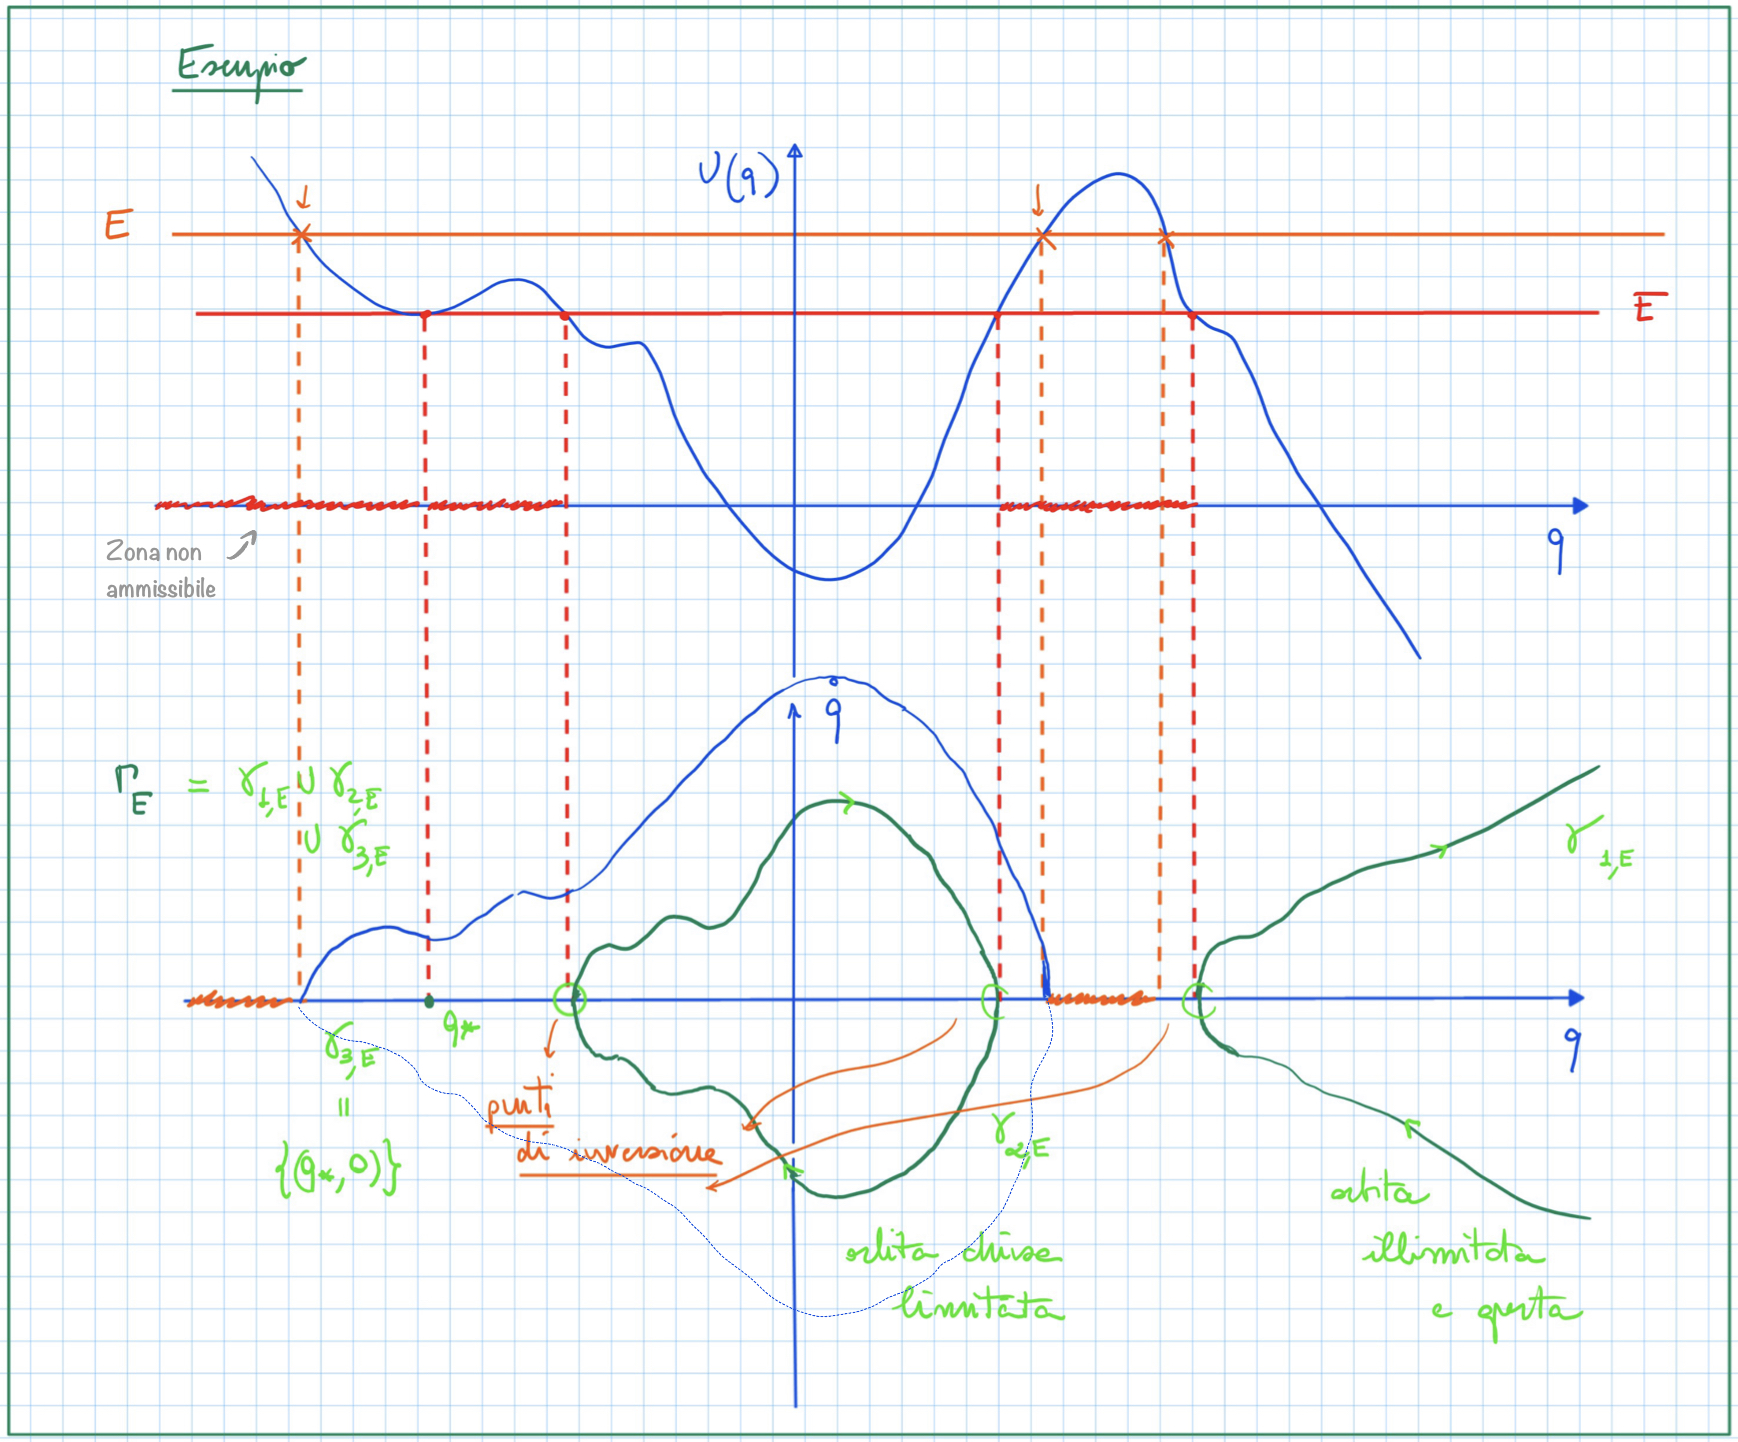
\includegraphics[width=13cm]{CurveLivello.jpeg}\\
\end{center}
\end{figure}
\newpage
%
%
%
Consideriamo ora i valori $E\in\Lambda_C$ t.c. E=U(q*), U'(q*)=0 \\
Oss: $U^{(n)}(q*)\neq 0 \Rightarrow$ \ 1) minimo se n pari e  $U^{(n)} > 0$ \ \ 2) massimo se n pari e $U^{(n)} < 0$ \ \ 3) flesso se n dispari 
%
%
%
\begin{wrapfigure}{r}{0.16\textwidth}
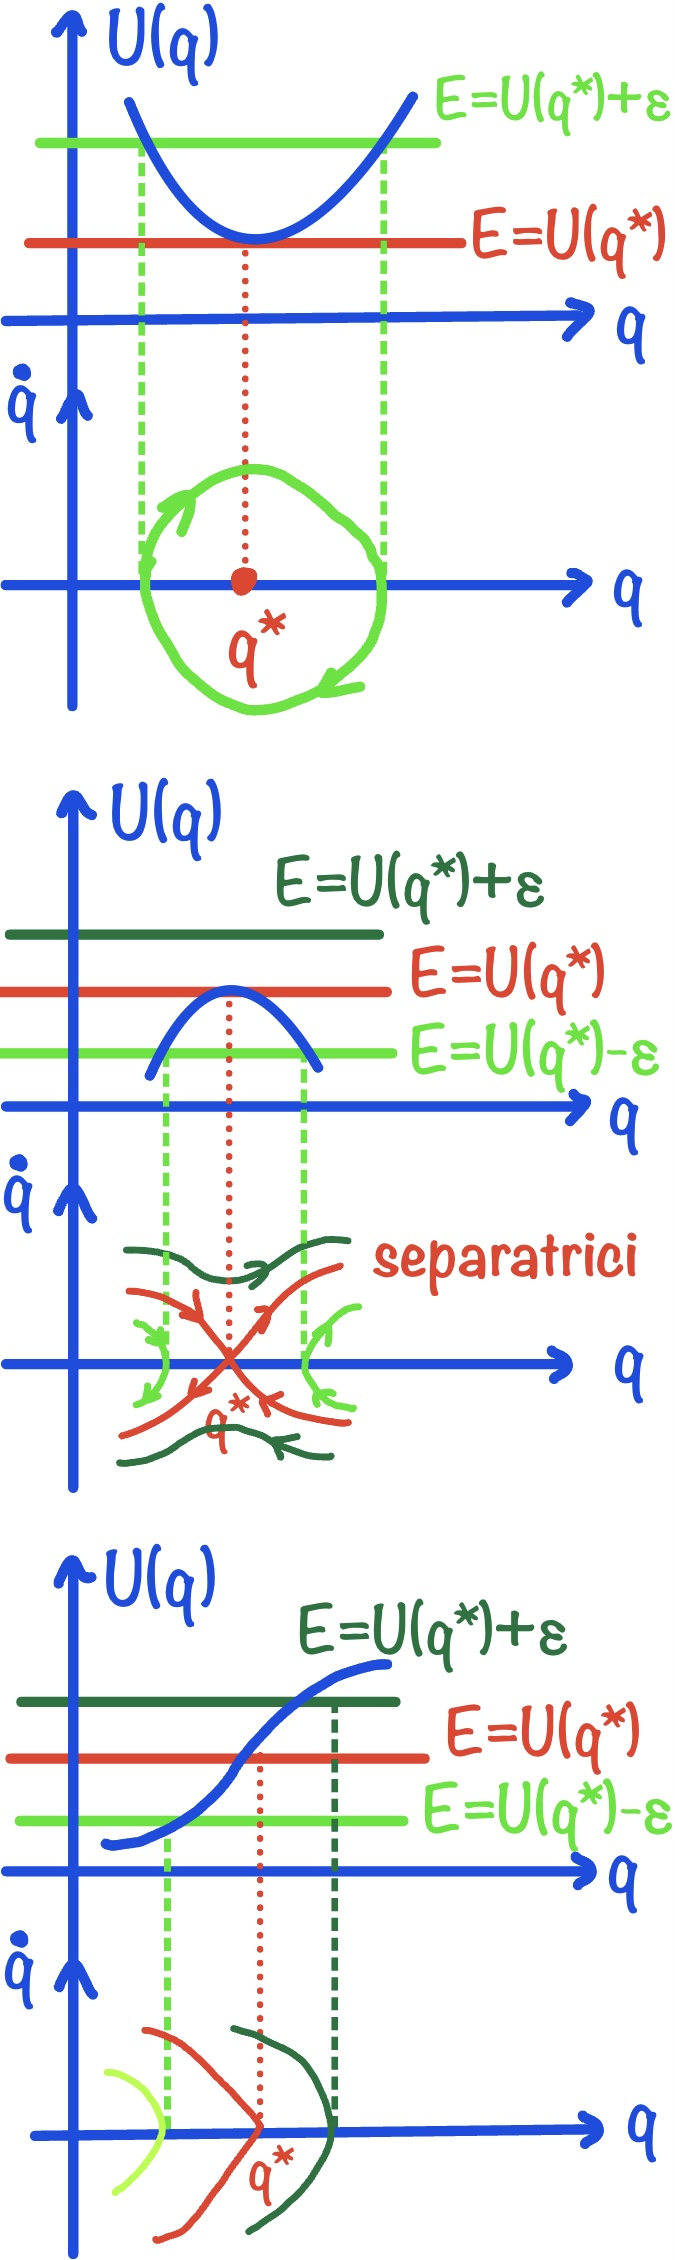
\includegraphics[width=0.16\textwidth]{PuntiCritici2.jpeg}
\end{wrapfigure}\\
%
%
\ • \ q* punto di \textbf{minimo isolato} di U \ \ \ \ stabile\\
\phantom{\ • }$\exists \gamma_E=\{(q*,0)\}$ orbita che corrisponde al solo punto di equilibrio\\
\phantom{\ • }Valori vicini di E producono orbite chiuse, limitate e periodiche \\ \\
%
%
\ • \ q* \textbf{massimo isolato} \ \ \ \ instabile\\
\phantom{\ • }$\exists \gamma_E=\{(q*,0)\}$ e per E=U(q*) $\exists\gamma_{*,j}\subset\Gamma_E$ 4 separatrici, disgiunte\\
\phantom{\ • }Valori di E vicini a U(q*) producono orbite che si allontanano da q*\\
Prop: Da ogni punto della separatrice, si raggiunge q* in tempo $\infty$ (+dim)\\ \\
%
\ • \ q* \textbf{flesso} ascendente o discendente \ \ \ \ instabile\\
\phantom{\ • }$\exists \gamma_E=\{(q*,0)\}$ e  per E=U(q*) $\exists \gamma_{*,j}\subset\Gamma_E$ 2 separatrici, disgiunte\\
\phantom{\ • }Valori vicini di E producono orbite lungo cui il sistema si allontana\\
Prop: La prolunga delle separatrici nel punto di eq non è verticale (+dim)\\

\subsection{Stabilità alla Lyapunov}
%
\begin{defi}
Un \textbf{sistema dinamico} è un problema di Cauchy: $\begin{cases} \dot{\overline{x}}=\overline{f}(\overline{x},\dot{\overline{x}},t)\\ \overline{x}(0)=\overline{x}_0 \end{cases}$  con $\overline{x}\in\mathbb{R}^n, \overline{f} \in C^{\infty} $
\end{defi}
%
\begin{defi}
Una configurazione $\overline{x}_0$ è di \textbf{equilibrio} se $\overline{f}(\overline{x}_0,\overline{0},t)=\overline{0}$
\end{defi}
%
%
%
\begin{Ndefi}
Stabilità alla \textbf{Ljapunov}: \ Una configurazione di equilibrio $\overline{x}_*$ di un sistema dinamico, sarà:\\
\ • \ \ \textbf{stabile} se $\forall \varepsilon>0, \exists\delta>0 : |\overline{x}(0)-\overline{x}_*|<\delta \implies |\overline{x}(t)-\overline{x}_*|<\varepsilon, \forall t\in \mathbb{R}^+$ \\
\ • \ \ \textbf{asintoticamente stabile} se stabile e $lim_{t\rightarrow +\infty} \overline{x}(t)=\overline{x}_*$\\
\ • \ \ \textbf{instabile} se non è stabile
\end{Ndefi}
%
Oss: Nel piano delle fasi le stabilità secondo Ljapunov di un punto di equilibrio equivale a:\\
\phantom{Oss: }Fissato il raggio $\varepsilon>0$ del disco $D_{\varepsilon}$ con centro q*, $\exists$ sempre un disco $D_{\delta}$ (in q* e raggio $\delta>0$) t.c. \\
\phantom{Oss: }$\forall \ (q(0),\dot{q}(0))\in D_{\delta} \implies (q(t),\dot{q}(t))\in D_{\varepsilon} \ \forall t \in \mathbb{R}$, \ cioè l'orbita non esce mai dal disco $D_{\varepsilon}$ \\ \\
% Si può aggiungere disegno esplicativo dell'oss
%
%
%Lezione18
%
Oss: Condizioni di equilibrio per sistemi olonomi conservativi sono del tipo $(\overline{q}_*,\overline{0})$\\
%
\phantom{Oss: }di conseguenza le condizioni diventano: $\ |\overline{q}(0)-\overline{q}_*|^2 + |\dot{\overline{q}}(0)|^2<\delta^2 \implies |\overline{q}(t)-\overline{q}_*|^2+|\dot{\overline{q}}(t)|^2<\varepsilon^2, \forall t \ $ \\
\phantom{Oss: }Ovvero partendo vicino a $q_*$ con velocità piccola si resta in un intorno del punto di equilibrio\\
%
Oss: Un sistema olonomo conservativo con matrice di massa A, avrà: \ $\overline{x}=(\overline{q},\overline{v}) \ \ \ \dot{\overline{x}}=(A^{-1}\overline{v},-\nabla U)$ \\  % ci vuole \\ \\, ma c'è nuova pagina
%
%
%
Oss: Il problema dinamico si può riscrivere \ $\dot{\overline{x}}=A(\overline{x}-\overline{x}_*)+Q(\overline{x})$ per sviluppo di Taylor con \ $lim_{\overline{x}\rightarrow\overline{x}_*}\frac{|Q(\overline{x})|}{|\overline{x}-\overline{x}_*|}$  \\
%
Oss: Dato un problema dinamico del tipo $\begin{cases}\dot{\overline{x}}=A\overline{x} \\ \overline{x}(0)=\overline{x}_0\end{cases}$ l'unica soluzione sarà \ $\overline{x}(t)=e^{At}\overline{x}_0$\\
%
Oss: L'esponenziale di una matrice è \ $e^{At}=\sum_{k=0}^{+\infty}\frac{(At)^k}{k!}$ e so che questa serie è ben definita \\
%
Oss: Se A è diagonalizzabile, allora $\exists$ base ortonormale t.c. il problema diventa $\dot{x}_j=\lambda_jx_j$\\
\phantom{Oss: }e la soluzione $x_j(t)=e^{\lambda_jt}(\overline{x}_0)_j$\\
%
Oss: In generale siano $\lambda_j$ gli autovalori di A e $n_j$ le corrispettive molteplicità, allora $\exists$ base t.c.\\
\phantom{Oss: }soluzioni sono: $x_j(t)=e^{\lambda_jt}P_j(t) \ \ P_j(t)=\sum_{k=0}^{n_j-1}c_kt^n$\\
%
%
%
\begin{defi}
Il \textbf{linearizzato} di (D) attorno a $\overline{x}_*$ punto di equilibrio è (L) \ $\begin{cases}\dot{\overline{x}}=A(\overline{x}-\overline{x}_*) \\ \overline{x}(0)=\overline{x}_0\end{cases}$ \ \ $A_{ij}=\frac{\partial f_i}{\partial x_j}(\overline{x}_*)$
\end{defi}
%
Teo: (Criterio linearizzato per stabilità) \ \ \ (+dim)\\
Dato (L) con $\lambda_j$ autovalori di A. \ Se $\exists$ c>0 t.c. $\mathcal{R}e\lambda \le -c <0 \ \forall \lambda_j$ \ allora $\overline{x}_*$ è un pt di eq asintoticamente stabile
ed $\exists$ una costante $C_0<+\infty$ e un intorno di $\overline{x}_* \  B(\overline{x}_*)$ t.c. \ $|\overline{x}(t)-\overline{x}_*| \le C_0 e^{-c\frac{t}{2}}|\overline{x}_0-\overline{x}_*| \ \ \forall \overline{x}_0 \in B(\overline{x}_*)$ \\
%
Lemma di Gronwall: \
Sia $g:\mathbb{R}\rightarrow\mathbb{R}^+, g\in C^1(\mathbb{R}) \ \ t.c. \ \exists k>0, \ \dot{g}\le kg \ \forall t \in \mathbb{R} \ \ \implies \ g(t)\le e^{kt}g(0)$ \ \ \ (+dim)\\ \\
%
%
%Lezione19
%
Cor: Se $\exists \lambda$ autovalore della matrice A del linearizzato t.c. $Re\lambda>0$ allora $\overline{x}_*$ è instabile\\
%
Oss: Il criterio linearizzato non funziona sempre (se $Re\lambda=0$)\\ \\
%
%
%
Teo: (Ljapunov) \ (+dim) \ \ \ \ Sia $\overline{x}_*$ un pt.\! di eq.\! del sistema dinamico (D). \\ Se esiste una funzione $W:\mathbb{R}^n\rightarrow\mathbb{R}$ (funzione di Ljapunov) definita in un intorno $B(\overline{x}_*)$ di $\overline{x}_*$ e di classe $C^1$ \\ Se valgono: \ \
i)$W(\overline{x}_*) = 0 , \ W(\overline{x})>0 \ \ \forall \overline{x} \in B(\overline{x}_*)/\{\overline{x}_*\}$ \ \ \
ii)$\dot{W}(\overline{x})\le 0 \ \ \forall \overline{x} \in B(\overline{x}_*) $ \ \ \ \ Allora $\overline{x}_*$ è stabile \\ \\
%
%
%
Oss: Se inoltre $\dot{W}(\overline{x})<0 \ \forall \overline{x}\in B(\overline{x}_*)/\{\overline{x}_*\}$ (Quindi $\dot{W}(\overline{x}_*)=0$) \ allora $\overline{x}_*$ asintoticamente stabile \\
%
Cor: Se invece \ ii)$\dot{W}(\overline{x}_*)\ge 0 \ \ e \ \dot{W}(\overline{x})>0 \ \ \forall \overline{x} \in B(\overline{x}_*)/\{\overline{x}_*\}$ \ \ allora $\overline{x}_*$ è instabile \ \ \ (+dim) \\
Oss: \ \ $\dot{W}(\overline{x})=\dot{\overline{x}}\cdot \nabla W = \overline{f}(\overline{x};\dot{\overline{x}};t)\cdot \nabla W(\overline{x}) $\\ \\
%
%
%
Teo: (Dirichlet) \ \ Dato un sistema olonomo conservativo\\ I punti di minimo isolati di U sono punti di equilibrio stabili del sistema \ \ \ (+dim)\\
%
Oss: Questa condizione è sufficiente ma non necessaria \\ \\
%
%
%
Prop: Per un sistema olonomo conservativo unidimensionale\\
\phantom{Prop: }se q* è un punto di massimo di U con U''(q*)<0, allora q* è instabile \ \ \ (+dim)\\
%
Oss: La generalizzazione multidimensionale richiede $\exists$ autovalore negativo di $Hess_U(\overline{q}*)$ \\





\section{Meccanica Lagrangiana}


\subsection{Equazioni di Lagrange}
%
\begin{defi}
La \textbf{Lagrangiana} di un sistema olonomo è:\\
\phantom{DEF: } $\mathcal{L}(\overline{q};\dot{\overline{q}};t):=T(\overline{q};\dot{\overline{q}};t) - U(\overline{q};t)$ \ \ \ \ \ con $T(\overline{q};\dot{\overline{q}};t)=\frac{1}{2}\dot{\overline{q}}A(\overline{q};t)\dot{\overline{q}} + \overline{b}(\overline{q};t)\cdot\dot{\overline{q}} + \overline{c}(\overline{q};t)$
\end{defi}
%
%Lezione20
%
Teo: (Equazioni di Eulero-Lagrange) \ \ \ (+dim)\\
Dato un sistema olonomo conservativo, \ $\overline{q}(t):[t_0,t_1]\rightarrow\mathbb{R}^g$ è un moto del sistema se e solo se sono soddisfatte le equazioni di Lagrange:  \ \ \ \ \ $\frac{d}{dt}\frac{\partial\mathcal{L}}{\partial\dot{q}_k} - \frac{\partial\mathcal{L}}{\partial q_k} = 0 \ \ \forall k \in \{1...g\}, \forall t \in (t_0,t_1) $\\
%
Lemma: Ponendo $\tau_k:=\sum_{j=1}^N m_j\overline{a}_j \cdot \frac{\partial \overline{x}_j}{\partial q_k} $ (componenti generalizzate delle forze inerziali)  \\
\phantom{Lemma: } si ha lungo ogni moto del sistema \ \ $\frac{d}{dt}\frac{\partial T}{\partial\dot{q}_k} - \frac{\partial T}{\partial q_k} = \tau_k$  \ \ \ (+dim)\\
%
Oss: Se le forze attive non sono conservative le eq. \! di Lagrange diventano:  \\
\phantom{Oss: }$\frac{d}{dt}\frac{\partial T}{\partial\dot{q}_k} - \frac{\partial T}{\partial q_k} = Q_k \ \ \forall k \in \{1...g\}$ \ \ \ $Q_k$ componenti generalizzate delle forze\\ \\
%
%
%
Oss: • se U è $C^2$ il moto ammette unica soluzione (essendo un sistema diff 2° ord) \\
\phantom{Oss: }• se $A(\overline{q})$ non dipende da t, allora $\frac{\partial\mathcal{L}}{\partial q_k}=\frac{1}{2}\dot{\overline{q}}\frac{\partial A(\overline{q})}{\partial q_k}\dot{\overline{q}}-Q_k$ \\
\phantom{Oss: }• se A non dipende da $\overline{q}$, allora $\ddot{\overline{q}}=A^{-1}\overline{Q}$ \\
%
Prop: (conservazione dell'energia) \ \ \ (+dim)\\
Se $\mathcal{L}(\overline{q};\dot{\overline{q}})=T(\overline{q};\dot{\overline{q}})-U(\overline{q})$ non dipende esplicitamente da t, $E=T(\overline{q};\dot{\overline{q}})+U(\overline{q})$ \ \ \ con $T(\overline{q};\dot{\overline{q}})=\frac{1}{2}\dot{\overline{q}}A(\overline{q})\dot{\overline{q}}$, allora E è un integrale primo del moto   (cioè $E(t)=E(0)+\dot{E}(0) \ t$)



\subsection{Simmetrie}
%
\begin{defi}
Una coordinata $q_k$ è \textbf{ciclica} per la Lagrangiana $\mathcal{L}(\overline{q};\dot{\overline{q}},t)$ se $\mathcal{L}$ non dipende da $q_k$ ovvero $\frac{\partial\mathcal{L}}{\partial q_k}=0$
\end{defi}
%
Prop: Sia $q_k$ una coordinata ciclica per $\mathcal{L}(\overline{q};\dot{\overline{q}},t)$, allora il \textbf{momento coniugato} $p_k=\frac{\partial \mathcal{L}}{\partial \dot{q}_k}$ \\
\phantom{Prop: }è un integrale primo del moto, cioè $\dot{p}_k=0$ \ \ \ (+dim)\\
%
%
%
\begin{Ndefi}
Una \textbf{simmetria} è una trasformazione $\overline{\Phi}:\mathbb{R}^g\rightarrow \mathbb{R}^g \ C^{\infty}$ invertibile t.c. $\mathcal{L}(\overline{q};\dot{\overline{q}})=\mathcal{L}(\overline{q}';\dot{\overline{q}'})$ \ \ $\overline{q}'=\overline{\Phi}(\overline{q})$\\
%
Un \textbf{gruppo ad un parametro di simmetrie} è una famiglia di diffeomorfismi $\{\overline{\Phi}_{\varepsilon}\}_{\varepsilon\in\mathbb{R}}:\mathbb{R}^g\rightarrow\mathbb{R}^g$ t.c.\\ Sia derivabile in $\varepsilon$, $\overline{\Phi}_{\varepsilon}$ simmetria $\forall \varepsilon$\ e\ \ \
i) $\overline{\Phi}_0(\overline{q})=\overline{q} \ \ \forall \overline{q}\in\mathbb{R}^g$ \ \ \ ii) $\overline{\Phi}_{\varepsilon_1}(\overline{\Phi}_{\varepsilon_2}(\overline{q}))=\overline{\Phi}_{\varepsilon_1+\varepsilon_2}(\overline{q}) \ \ \forall \varepsilon_1, \varepsilon_2\in\mathbb{R}$
\end{Ndefi}
%
%
%
Teo: (Noether) \ \ \ (+dim) \\
Se un sistema di Lagrangiana $\mathcal{L}(\overline{q};\dot{\overline{q}})$ ammette una famiglia ad 1 parametro di simmetrie $\{\overline{\Phi}_{\varepsilon}\}_{\varepsilon\in\mathbb{R}}$,\\
Allora la seguente quantità è un integrale primo del moto: \ \ \ \ $I(\overline{q};\dot{\overline{q}})=\nabla_{\dot{\overline{q}}}\mathcal{L}\cdot\frac{\partial\Phi_{\varepsilon}}{\partial\varepsilon}|_{\varepsilon=0}=\sum_{k=1}^g\frac{\partial\mathcal{L}}{\partial\dot{q}_k}\cdot \frac{\partial(\Phi_{\varepsilon})_k}{\partial\varepsilon}|_{\varepsilon=0}$ \\
Oss: Esistono integrali primi del moto che non derivano dalla presenza di simmetrie\\
%
Oss: Conseguenza di Noether è che la simmetria per rotazioni attorno ad un asse implica\\
\phantom{Oss: }la conservazione del momento angolare lungo quell'asse





\subsection{Moti Centrali}
%
Consideriamo sistema di due corpi in interazione interna con una forza \ \ $\overline{F}_{ij}=f(|\overline{x}_1-\overline{x}_2|)\hat{x}_{ij}$\\
Prop: Nelle coordinate $\overline{X}:=\frac{m_1\overline{x}_1+m_2\overline{x}_2}{m_1+m_2}$ e $\overline{r}:=\overline{x}_1-\overline{x}_2$, la Lagrangiana del sistema è: \\
\phantom{Prop: }$\mathcal{L}(\overline{X};\dot{\overline{X}};\overline{r};\dot{\overline{r}})=\frac{1}{2}(m_1+m_2)|\dot{\overline{X}}|^2+\frac{1}{2}\mu|\dot{\overline{r}}|^2 -U(|\overline{r}|)$ \\
\phantom{Prop: }dove $\mu=(\frac{1}{m_1}+\frac{1}{m_2})^{-1}$ è la massa ridotta e U una primitiva di -f (cioè $U'=-f$) \ \ \ (+dim)\\
%
Oss: Lagrangiana ciclica rispetto $\overline{X} \implies \overline{p}_X:=(m_1+m_2)\dot{\overline{X}}$ (momento totale) è integrale primo del moto.\\ \phantom{Oss: }Quindi esiste un osservatore solidale al centro di massa, rispetto ad esso $\mathcal{L}=\mathcal{L}(\overline{r};\dot{\overline{r}})=\frac{1}{2}\mu|\Dot{\overline{r}}|^2 - U(|\overline{r}|)$ \\ \\ 
%
%
%
%Lezione21
%
Oss: $\mathcal{L}$ non dipende esplicitamente dal tempo $\implies E=\frac{1}{2}\mu|\Dot{\overline{r}}|^2 + U(|\overline{r}|)$ \ \ è integrale primo del moto \\
%
Prop: Il momento angolare \ $\overline{L}:=m\overline{r}\wedge\Dot{\overline{r}}$ è un integrale primo (in 3D) del moto \ \ \ (+dim)\\ \\
%
%
%
Oss: In un campo centrale \ $\mathcal{L}(\overline{r};\Dot{\overline{r}})=\frac{1}{2}\mu|\Dot{\overline{r}}|^2 -U(|\overline{r}|)$  \ e \ $\overline{F}(\overline{r})=-U'(|\overline{r}|)\hat{r}$\\
%
Prop: Il moto di un sistema in un campo centrale è: \\
\phantom{Prop: }i) rettilineo se $\overline{L}(0)=\overline{0}$ \ \ \ ii) piano se $\overline{L}(0)\neq \overline{0}$\ \ (sul piano $\perp$ a $\overline{L}(0)$) \ \ \ (+dim)\\
%
%
%
\begin{defi}
La \textbf{velocità areolare} $\Dot{A}(t)$ è la derivata sul tempo dell'area coperta dalla traiettoria al variare di t
\end{defi}
Teo: (II legge di Keplero) In un campo centrale la velocità areolare $\Dot{A}(t)$ è costante \ \ \ (+dim)\\ \\
%
%
%
Oss: In coordinate polari $\mathcal{L}(\rho;\theta;\dot{\rho};\dot{\theta}) = \frac{1}{2}\mu (\dot{\rho}^2+\rho^2 \dot{\theta}^2) -U(\rho)$\\
%
Prop: Ogni moto centrale con $L\neq0$ si decompone in: \ \ \ \ \ \ (+dim)\\
\phantom{Prop: }i) un moto radiale unidimensionale in $\rho$ con energia conservata $E=\frac{1}{2}\mu\Dot{\rho}^2 +U_{eff}(\rho) $ \\
\phantom{Prop: i) }dove il potenziale efficace è $U_{eff}(\rho)=\frac{L^2}{2\mu\rho^2}+U(\rho) $\\
\phantom{Prop: }ii) un moto angolare unidimensionale in $\theta(t)$ soluzione di $\Dot{\theta}=\frac{L}{\mu\rho^2(t)} $ \\
\phantom{Prop: ii) }Inoltre la curva nel piano $\rho,\theta$ ha eq.\! soluzione di $\frac{d\rho}{d\theta}=\pm \frac{\mu\rho^2}{L}\sqrt{\frac{2}{\mu}(E-U_{eff}(\rho))}$ \\ \\
%
%
%
Prop: Se $E\in\Lambda_C(U_{eff})$ (non asintoto), allora una soluzione del moto è $\rho(t)=\rho_* $\\
\phantom{Prop: }il moto complessivo è circolare uniforme $ \ \theta(t)=\theta_0+\omega t$ \ con \ $\omega=\frac{L}{\mu\rho_*^2}$ \\
%
Prop: Se $E\notin\Lambda_C(U_{eff})$ e $lim_{\rho\rightarrow0^+}\ \rho^2U(\rho)=0$, \ il moto si svolge all'interno di $[\rho_m,+\infty)\ \ \rho_m>0$ \ \ \ (+dim)\\
%
Oss: Le orbite radiali limitate per $E\notin\Lambda_C(U_{eff})$ sono chiuse e periodiche \\ \\
%
%
%
Prop: Un moto centrale è periodico se e solo se \ \ \ \ \ (+dim)\\
\phantom{Prop: }i) il moto radiale è periodico di periodo T oppure di quiete \\
\phantom{Prop: }ii) la variazione di $\theta$ di un T soddisfa \ \ $\Delta\theta := \theta(T)-\theta(0) = \int_0^T\frac{L^2}{\mu\rho^2(\tau)}d\tau=\frac{p}{q}2\pi$ \ \ con $p,q\in\mathbb{Z}^+$ \\
\phantom{Prop: ii) }e in tal caso il periodo complessivo è nT con n il più piccolo q t.c.\! la condizione è soddisfatta \\
%
Oss: Ogni orbita radiale che non corrisponda a valori critici dell'energia è periodica ma la condizione non è soddisfatta, allora l'orbita è aperta e limitata nella corona circolare di raggi $\rho_-, \rho_+$ punti di inversione



%Lezione22

\subsection{Campo Gravitazionale}
%
\begin{wrapfigure}{r}{0.24\textwidth}
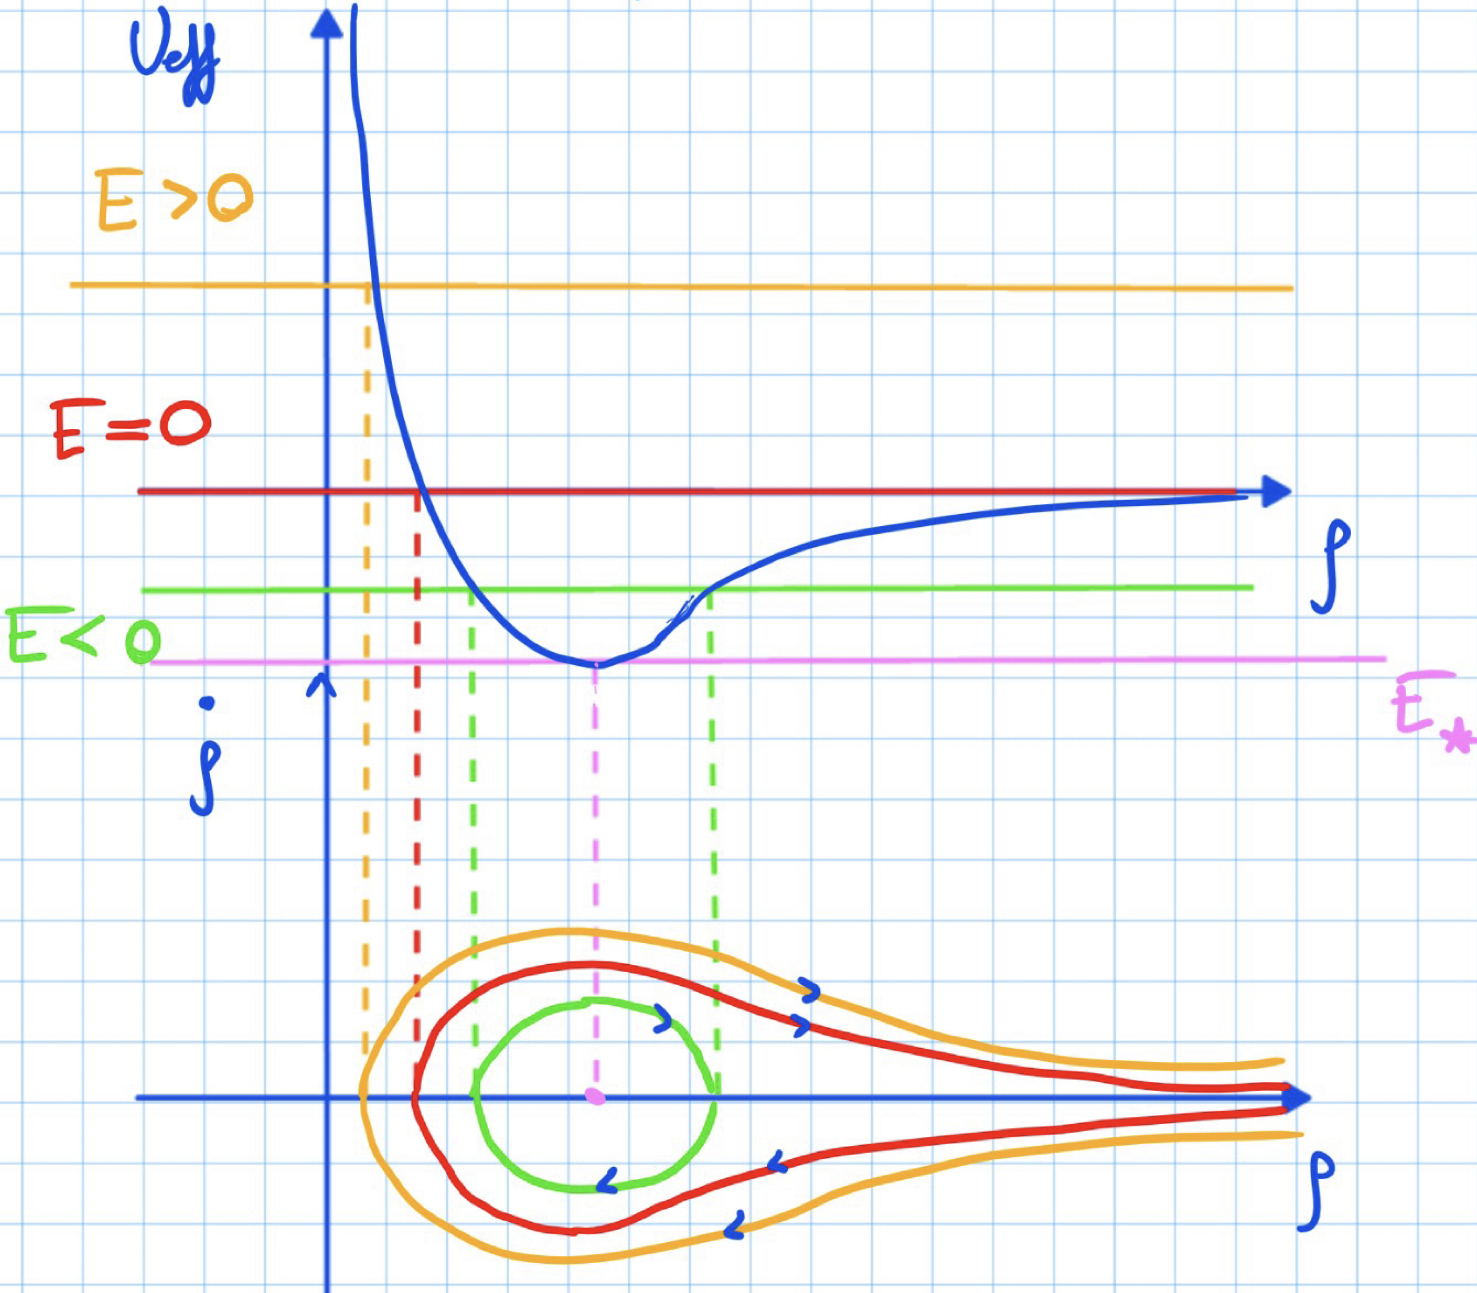
\includegraphics[width=0.24\textwidth]{CampoGravitazionale.jpeg}
\end{wrapfigure}
Nel campo gravitazionale valgono:\\
\ • \ \ $U(\rho)=-\frac{k}{\rho} \ \ \ \ U_{eff}(\rho)=\frac{L^2}{2m\rho^2}-\frac{k}{\rho} \ \ \ k>0$\\
\ • \ \ $min U_{eff}(\rho)=U_{eff}(\rho_*)=-\frac{k^2m}{2L^2}=E_*$\\
\ • \ \ $\rho_*=\frac{L^2}{km}$  è un pt.\! di minimo assoluto \\
\ • \ \ i valori ammissibili sono $E\in[E_*,+\infty)$ e quelli critici $\Lambda_C$=\{0,$E_*$\}\\
\ • \ \ l'eccentricità è $e:=\sqrt{1-\frac{E}{E_*}}$\\ \\
%
%
%
Prop: L'eq.\! delle orbite in un campo gravitazionale è:  $\rho(\theta)=\frac{\rho_*}{1+e\cdot cos(\theta)}$ \ \ \ \ \ (+dim)\\
\phantom{Prop: }Di conseguenza le orbite sono: \ \ \ i) ellissi se $e<1$ \ \ \ ii) parabole se $e=1$ \ \ \ iii) iperboli se $e>1$\\
\phantom{Prop: }In particolare, le orbite limitate ($e<1$) sono periodiche con periodo T del moto radiale \\
Oss: Il tipo di una conica di eq. $\overline{x}A\overline{x}=0$,    è dato dal determinante della sottomatrice $\begin{pmatrix}a_{11} \ a_{12} \\ a_{21} \ a_{22}\end{pmatrix}$  \\ \\
%
%
%
Teo: (Leggi di Keplero) \ \ \ (+dim.)\\
Per ogni moto in un campo gravitazionale, valgono:\\
i) le orbite sono ellissi, in cui il centro della forza occupa uno dei due fuochi\\
ii) la velocità areolare è costante\\
iii) il quadrato del periodo dell'orbita è proporzionale al cubo del semiasse maggiore \ \ $T^2\propto a^3$\\ \\
%
%
%
Oss: Le traiettorie ellittiche hanno un fuoco in O, quindi asimmetriche $\implies T=T_{radiale}$ e $\Delta\theta=2\pi$\\
%
Oss: Per l'oscillatore armonico, le orbite ellittiche sono simmetriche con centro in O $\implies T=2T_{radiale}$\\
%
Oss: Sia per il campo gravitazionale che per l'oscillatore, tutte le orbite limitate sono anche periodiche \\ \\
%
%
%
Teo: In un campo centrale tutte le orbite limitate sono chiuse $\Longleftrightarrow \ U(\rho)=\begin{cases} \frac{1}{2}k\rho^2 \ \text{ oscillatore armonico}\\ -\frac{k}{\rho} \ \ \ \text{ campo gravitazionale} \end{cases}$\\
%
Oss: Per un potenziale centrale generico (non gravitazionale o armonico)\\
\phantom{Oss: }l'insieme dei dati iniziali che generano orbite chiuse ha misura di Lebesgue nulla \\ \\
%
%
%
I potenziali gravitazionale e armonico sono particolari perché hanno più simmetrie dei campi centrali generici\\
Prop: Per ogni moto in un campo gravitazionale il \textbf{vettore di Runge-Lenz} \\
\phantom{Prop: }$\overline{R}= m(\dot{\overline{x}}\wedge\overline{L}-k\hat{r})$ è un integrale primo del moto \ \ \ (+dim)


%Lezione23
\subsection{Piccole Oscillazioni}
%
Consideriamo il sistema olonomo conservativo di Lagrangiana \ \ $\mathcal{L}(\overline{q};\dot{\overline{q}})=\frac{1}{2}\dot{\overline{q}}A(\overline{q})\Dot{\overline{q}} -U(\overline{q}) \ \ \overline{q}\in\mathbb{R}^g$\\
Prop: Il sistema dinamico linearizzato attorno  un pos.\! di eq.\! stabile $\overline{q}_*$ del sistema olonomo conservativo\\
\phantom{Prop: }ha equazioni del moto \ $A\Ddot{\overline{u}}= -B\overline{u}$ \ ed è descritto dalla Lagrangiana \ $\widetilde{\mathcal{L}}(\overline{u};\dot{\overline{u}})=\frac{1}{2}\Dot{\overline{u}}A\Dot{\overline{u}} -\frac{1}{2}\overline{u}B\overline{u}$ \\
\phantom{Prop: }dove $A=A(\overline{q}_*)$ \ \ $B= Hess_U(\overline{q}_*)$ \ \ $\overline{u}=\overline{q}-\overline{q}_*$ \ \ \ \ \ (+dim) \newpage  %altrimenti ci vuole \\
%
%
%
\begin{defi}
Le \textbf{piccole oscillazioni} rispetto a $\overline{q}_*$ stabile sono i moti descritti dalla Lagrangiana $\widetilde{\mathcal{L}}$ del\\ linearizzato.
Ogni singola oscillazione e la sua frequenza sono dette modo normale e frequenza propria
\end{defi}
%
%
%
Teo: (piccole oscillazioni) \ \ \ (+dim)\\
Dato il sistema linearizzato con $B>0$ i modi normali sono: \ \ $z_i(t)=z_i(0)cos\omega_it+\frac{\dot{z}_i(0)
}{\omega_i}sen\omega_it \ \ \ i\in\{1...g\}$ \\
Le relative frequenze proprie $\omega_i$ sono soluzioni dell'equazione caratteristica \ $det(B-\omega^2A)=0$ \\
Più precisamente $\exists C=(\overline{\xi}_1|...|\overline{\xi}_g)$ \ t.c. la soluzione del moto è data da $\overline{u}(t)=C\overline{z}(t)$ \ con $\overline{\xi}_i$ t.c. $(B-\omega_i^2A)\overline{\xi}_i=0$\\ \\
%
%
%
Oss: Le piccole oscillazioni hanno la forma $\overline{u}(t)=\sum_{i=1}^gz_i(t)\overline{\xi}_i$\\
Lemma1: Per A,B simmetriche con A>0, \ $\exists$ C invertibile t.c. $CAC^{-1}= \mathds{1} $, \ $CBC^{-1}=diag(\beta_1...\beta_g)$ \ \ \ (+dim)\\
Cor: Le soluzioni del linearizzato corrispondono a vere oscillazioni $\Longleftrightarrow\omega_i>0 \ \forall i$, \ altrimenti $\overline{q}_*$ è instabile\\
Lemma2: A,B simmetriche A>0, gli autovalori $\varepsilon_i$ di $A^{-\frac{1}{2}}BA^{-\frac{1}{2}}$ sono le soluzioni di $det(B-\lambda A)=0$ \ (+dim)\\ 



%Lezione24


\section{Meccanica Hamiltoniana}

\subsection{Principi Variazionali}
%
Mostriamo che la descrizione lagrangiana di un sistema olonomo conservativo si può ricavare da un principio variazionale, senza passare dalle equazioni di Newton\\
%
\begin{Ndefi}
Lo \textbf{spazio delle traiettorie} è: \ \ \ $\mathcal{M}_{\overline{q}_0,\overline{q}_T,T}:=\{\overline{q}(t):[0,T]\rightarrow \mathbb{R}^d \ |\ \overline{q}(0)=\overline{q}_0,\ \overline{q}(T)= \overline{q}_T , \ \overline{q}\in C^1([0,T])\}$\\
Lo \textbf{spazio delle deformazioni} è: \ \ \ $\mathcal{M}_{0,T}:=\{\overline{\eta}(t):[0,T]\rightarrow \mathbb{R}^d \ |\ \overline{\eta}(0)=\overline{\eta}(T)=0, \ \overline{\eta}\in C^1([0,T])\}$
\end{Ndefi}
%
%
%
\begin{Ndefi}
Sia X uno spazio vettoriale normato, un \textbf{funzionale} è un'applicazione $\mathcal{F}[f]:X\rightarrow \mathbb{R}$\\
%
Un funzionale $\mathcal{F}$ ha un \textbf{estremale} in $f_0$ se $\exists$ un intorno U di $f_0$ t.c. $sign(\mathcal{F}[f]-\mathcal{F}[f_0])$ è lo stesso $\forall f \in U$

(minimo se $\ge0$, massimo se $\le0$)
\end{Ndefi}
%
%
%
\begin{Ndefi}
Un funzionale continuo $\mathcal{F}$ è \textbf{differenziabile} in $f$ se \ $\Delta\mathcal{F}[\eta]:= \mathcal{F}[f+\eta]-\mathcal{F}[f] = \delta\mathcal{F}[f](\eta) + \varepsilon(\eta)||\eta|| \ \forall \eta$

dove $\delta\mathcal{F}$ è una funzione lineare, detta differenziale \ e \ $\lim_{||\eta||\to 0^+}\varepsilon(\eta)=0$
\end{Ndefi}
%
Teo: Se $\mathcal{F}$, differenziabile  in $X_0$, ha un estremale in $f\in X_0 $, allora \\
\phantom{Teo: }$\delta\mathcal{F}[f](\eta)=0 \ \forall \eta \in X_0$ \ cioè f è un punto stazionario di $\mathcal{F}$ \ \ \ (+dim) \\ \\
%
%
%
Consideriamo ora i funzionali $\mathcal{F}[f]:=\int_a^bF(f;f';x)dx$ con $F\in C^2$ e $f\in X=\{f\in C^1[a,b] \ |\ f(a)=f(b)=0 \}$\\
%
Teo: (equazioni di Eulero-Lagrange) \ \ \ (+dim)\\
$\mathcal{F}$ differenziabile in X ha un punto stazionario in $f_0\in X \Longleftrightarrow \frac{d}{dx}\frac{\partial F}{\partial f'}-\frac{\partial F}{\partial f}|_{f=f_0}=0 \ \ \forall x \in [a,b]$ \\
Lemma: Sia $g\in C[a,b]$ t.c. $\int_a^bg(x)f(x)dx=0 \ \ \forall f\in X$ \ \ allora g=0 \ \ \ (+dim)\\ \\
%
%
%
Oss: La generalizzazione a $\mathbb{R}^d$ è ovvia: \ \ $\frac{d}{dx}\frac{\partial F}{\partial f'_k}-\frac{\partial F}{\partial f_k}=0 \ \ \forall k $\\
%
Oss: La generalizzazione a funzionali $\mathcal{F}[\overline{f}], \ \overline{f}\in X$ affine su $X_0$ \ con $X=\{\overline{f}\in C^2[a,b] \ |\ \overline{f}(\overline{a})=\overline{A}, \ \overline{f}(\overline{b})=\overline{B}\}$ \\
%
%
%
\begin{defi}
Il \textbf{funzionale d'azione} è il funzionale sullo spazio affine $\mathcal{M}_{\overline{x}_0,\overline{x}_T,T}$ dato da \ \ $\mathcal{A}(\overline{q}):=\int_0^T\mathcal{L}(\overline{q};\dot{\overline{q}};t)dt$
\end{defi}
%
Teo: (Princio di Hamilton) \ \
Assumendo T e U $C^2$ \\ ogni moto del sistema olonomo conservativo rende stazionario il funzionale d'azione,\\ cioè se $\overline{q}_{ol}(t) $ risolve l'eq del moto in [0,T], allora $\delta\mathcal{A}[\overline{q}_{ol}]=0$ \ \ \ (+dim) \\ \\
%
%
%Lezione25
%
Teo: (Principio di minima azione) \ \ Assumendo T,U $\in C^2$ e $\frac{\partial^2T}{\partial\dot{q}_j\partial\dot{q}_k}>0$ \ (come matrice) \\
$\exists T>0 $ t.c. \ \ se $\overline{q}(t)$ rende stazionaria $\mathcal{A}[\overline{q}]$ in [0,T]
allora $\mathcal{A}[\overline{q}]$ ha un minimo relativo in $\overline{q}$  \ \ \ (+dim)\\ \\
%
%
%
Teo: Sia $X_{\mathcal{G}}:=\{ \overline{f}\in C^2([a,b]) \ |\ \overline{f}(a)=\overline{A}, \ \overline{f}(b)=\overline{B}, \ \mathcal{G}[\overline{f}]=l \in \mathbb{R} \}$ \\
\phantom{Teo: }dove $\mathcal{G}[\overline{f}]:=\int_a^bG(\overline{f};\overline{f}';x)dx$ con $G\in C^2$ (Vincolo) \ \ \
Allora, posto $\lambda\in\mathbb{R}$ \textbf{moltiplicatore di Lagrange} \\
\phantom{Teo: }$\overline{f}_0$ è un pt.\! stazionario di $\mathcal{F}[\overline{f}]:=\int_a^bF(\overline{f};\overline{f}';x)dx$ su $X_{\mathcal{G}} \Longleftrightarrow \overline{f}_0$ pt.\! stazionario di $\mathcal{F}[\overline{f}]+\lambda\mathcal{G}[\overline{f}] $


\subsection{Equazioni di Hamilton}
%
\begin{defi}
La \textbf{trasformata di Legendre} di $f(\overline{x})\in C^2$ convessa ($det\frac{\partial^2f}{\partial x_j\partial\ x_k}>0$) è \ $g(\overline{p}):=sup_{\overline{x}\in\mathbb{R}} \{\overline{p}\cdot\overline{x}-f(\overline{x})\} $
\end{defi}
%
Oss: Se sup=max allora $\exists \overline{x}(\overline{p})$ t.c. $g(\overline{p})=\overline{x}(\overline{p})\overline{p} -f(\overline{x}(\overline{p}))$, cioè $\nabla_{\overline{x}}(\overline{x}\overline{p} -f(\overline{x}))|_{\overline{x}(\overline{p})}=0 \implies \overline{p}=(\nabla f)(\overline{x}(\overline{p}))$ \\
%
Oss: Se f è $C^2$ e strettamente convessa $\forall \overline{x}\in\mathbb{R}^d$, allora il sup è il max (cioè non ci sono asintoti obliqui)\\
Oss: se d=1 \ \ $p=f'(x(p))$ \ \ la pendenza della tangente alla funzione in x\\ \\
%
%
%
Prop: La trasformata di Legendre g è $C^2$, convessa e involutiva, cioè f è la trasformata di g \ \ \ (+dim)\\
Oss: Inoltre se f è $C^k$ con $k>2 \implies$ g è $C^k$\\
%
%
%
\begin{defi}
L'\textbf{Hamiltoniana} è la trasformata rispetto $\dot{\overline{q}}$ di una Lagrangiana $H(\overline{q};\overline{p};t):=sup_{\overline{\eta}\in\mathbb{R}^g}\{\overline{p}\overline{\eta}-\mathcal{L}(\overline{q};\overline{\eta};t) \}$\\
Chiamiamo $p_k=\frac{\partial\mathcal{L}}{\partial\dot{q}_k}(\overline{q};\dot{\overline{q}}(\overline{p});t)$ il momento coniugato di $q_k$ e la coppia $(\overline{q},\overline{p})$ variabili canoniche
\end{defi}
%
%
%
Prop: Sia $\mathcal{L}(\overline{q};\dot{\overline{q}})=\frac{1}{2}\dot{\overline{q}}A(\overline{q})\dot{\overline{q}}-U(\overline{q}) \ \ (A,U\in C^2 \text{ e } A>0)$, allora $H(\overline{q};\overline{p})=\frac{1}{2}\overline{p}A^{-1}(\overline{q})\overline{p}+U(\overline{q})$ \ \ \ (+dim)\\
%
%
%
\begin{defi}
Le \textbf{equazioni di Hamilton} sono il sistema di eq.\! differenziali $(H): \ \ \begin{cases}
    \dot{q}_k=\frac{\partial H}{\partial p_k}\\
    \dot{p}_k=-\frac{\partial H}{\partial q_k}
\end{cases}$
\end{defi}
%
Prop: Sia $(\overline{q}(t),\overline{p}(t))$ una soluzione delle eq.\! di Hamilton, allora $\frac{d}{dt}H(\overline{q}(t);\overline{p}(t);t)=\frac{\partial H}{\partial t}(\overline{q}(t);\overline{p}(t);t)$ \ \ \ (+dim)\\
%
Cor: Se H non dipende esplicitamente da t, allora $\frac{dH}{dt}=0$ \ (H è integrale primo) \\ \\
%
%
%Lezione26
%
Oss: Il \textbf{flusso hamiltoniano} è la funzione: $t\rightarrow (\overline{q}(t),\overline{p}(t))$\\
%
Oss: Le equazioni di Hamilton sono formalmente equivalenti a quelle di Lagrange \\ \\
%
%
%
Oss: L'insieme delle $(\overline{q},\overline{p})$ è detto spazio delle fasi $\Gamma$ e può essere dotato di una struttura \textbf{simplettica}\\
%
Oss: Le eq di H \ $\dot{\overline{x}}=\overline{f}_H (\overline{x};t)$ si possono riscrivere con la matrice simplettica standard $J=\begin{pmatrix}
    \ 0 \ \ \mathds{1} \\
    -\mathds{1} \ \ 0
\end{pmatrix} \in M_{2g}$\\
\phantom{Oss: }e il campo vettoriale Hamiltoniano \ $\overline{f}_H (\overline{x};t) := J \ \nabla_{\overline{x}}H =(\nabla_{\overline{q}}H , -\nabla_{\overline{p}}H) $ \\ \\
%
%
%
Oss: Come per eq di $\mathcal{L}$, da quelle di H si ottengono dalla stazionarietà di \ $\mathcal{A}[(\overline{q},\overline{p})]:=\int_0^T\{\overline{p}\cdot\dot{\overline{q}}(\overline{p}) - H(\overline{q};\dot{\overline{q}};t)\}dt$ \\
\phantom{Oss: }nello spazio delle traiettorie \ $\mathcal{N}_{\overline{q}_0,\overline{q}_T,T}:=\{ (\overline{q},\overline{p}) \ | \ \overline{q}(0)=\overline{q}_0 , \ \overline{q}(T)=\overline{q}_T \}$ \\
Oss: H è definita a meno di C additiva ($\mathcal{L}$ a meno di $\dot{f}(t)$) \\ \\
%
%
%
Teo: (Liouville) \ \ \ (+dim)\\
Il flusso hamiltoniano conserva il volume nello spazio delle fasi, cioè $\forall \mathcal{D}\subset\Gamma, \ \ |\mathcal{D}_t|=|\mathcal{D}|$ \\
dove $\mathcal{D}_t:=\{ (\overline{q}(t),\overline{p}(t)) \ | \ \exists (\overline{q}_0,\overline{p}_0)\in \mathcal{D} \text{ e } (\overline{q}(0),\overline{p}(0))=(\overline{q}_0,\overline{p}_0)  \}$ \\
Oss: Qualunque sistema dinamico $\dot{\overline{x}}=\overline{f}(\overline{x};t)$ conserva il volume se $\overline{f}$ è a divergenza nulla \\ \\
%
%
%
Teo: (Eterno ritorno di Poincarrè) \ \ \ (+dim)\\
Sia $\overline{x}(t)$ un flusso Hamiltoniano t.c. $\overline{x}(\cdot\ ;t): \Omega \rightarrow \Omega$ con $\Omega \subset \Gamma$ compatto. \\
Allora $\forall B\subset\Omega$ palla aperta e $\forall t>0 \ \exists\overline{t}>t$ t.c. $B_{\overline{t}}\cap B \neq \emptyset$ \\
%
Cor: $\forall \overline{x}_0\in\mathcal{D}$ la traiettoria deve tornare in $\mathcal{D}$ infinite volte (a meno di un insieme a misura nulla) \ \ \ (+dim)\\
%
Oss: Non esistono equilibri asintoticamente stabili\\ 
%
Esempio: Diavoletto di Maxwell


\section{Esempi di sistemi meccanici}

\subsection{Moti rigidi liberi}
%
Prop: Dato un corpo rigido con punto fisso O, in assenza di forze esterne, $\dot{\overline{K}}_O'=\overline{K}_O'\wedge\overline{\omega}$ \\ 
\phantom{Prop: }con $\overline{K}_O'$ = momento angolare rispetto ad O misurato sul sistema solidale \ \ \ (+dim)\\
%
Cor: Usando come sistema solidale quello fissato dagli assi principali di inerzia,\\
\phantom{Cor: }le eq del moto prendono la forma delle equazioni di Eulero \ $\begin{cases}
I_1\dot{\omega}_1=(I_2-I_3)\omega_2\omega_3 \\
I_2\dot{\omega}_2=(I_3-I_1)\omega_1\omega_3\\
I_3\dot{\omega}_3=(I_1-I_2)\omega_1\omega_2
\end{cases}$ \\
%
%
%Lezione27
%
Oss: Se il sistema non è libero, ma sottoposto a forze esterne di momento $\overline{M}_0$ \ \ \ (E')=$\begin{cases}
I_1\dot{\omega}_1=(I_2-I_3)\omega_2\omega_3 + M_1 \\
I_2\dot{\omega}_2=(I_3-I_1)\omega_1\omega_3 +M_2\\
I_3\dot{\omega}_3=(I_1-I_2)\omega_1\omega_2 +M_3
\end{cases}$ \\ \\ %ce ne vorrebbe solo uno, ma cambio pagina
%
%
Prop: Sono integrali primi del moto le quantità: \ \ \ (+dim) \\
\phantom{Prop: }Energia \ $ E=\frac{1}{2}\sum_{j=1}^3I_j\omega_j^2 = \frac{1}{2}\sum_{j=1}^3\frac{K_j^2}{I_j}$\\
\phantom{Prop: }Momento angolare \ $|\overline{K}'_0|=\sum_{j=1}^3 K_j^2=\sum_{j=1}^3I_j^2\omega_j^2$ \\ \\
%
Prop: I moti si svolgono sull'intersezione dell'ellissoide di inerzia $\overline{K'}_0\mathbb{I}^{-1}\overline{K'}_0=2E$ e la sfera $|\overline{K'}_0|^2=cost$ \\
%
%
%
Le \textbf{rotazioni stazionarie} sono le soluzioni di (E) in cui $\overline{\omega}=cost$\\
%
%
Prop: Ogni corpo rigido con punto fisso O in assenza di forze esterne ammette rotazioni stazionarie attorno\\
\phantom{Prop: }a ciascun asse di inerzia \ \ \ (+dim)\\ \\
%
%
%
Vediamo in generale tutti i moti possibili in assenza di forze esterne, dividendo in 3 casi:\ \ \ \ \ \ \ \ \ \ \ \ \ \ \ \ \ \ \ \ \ \ \ \ \ \
\begin{wrapfigure}{r}{0.23\textwidth}
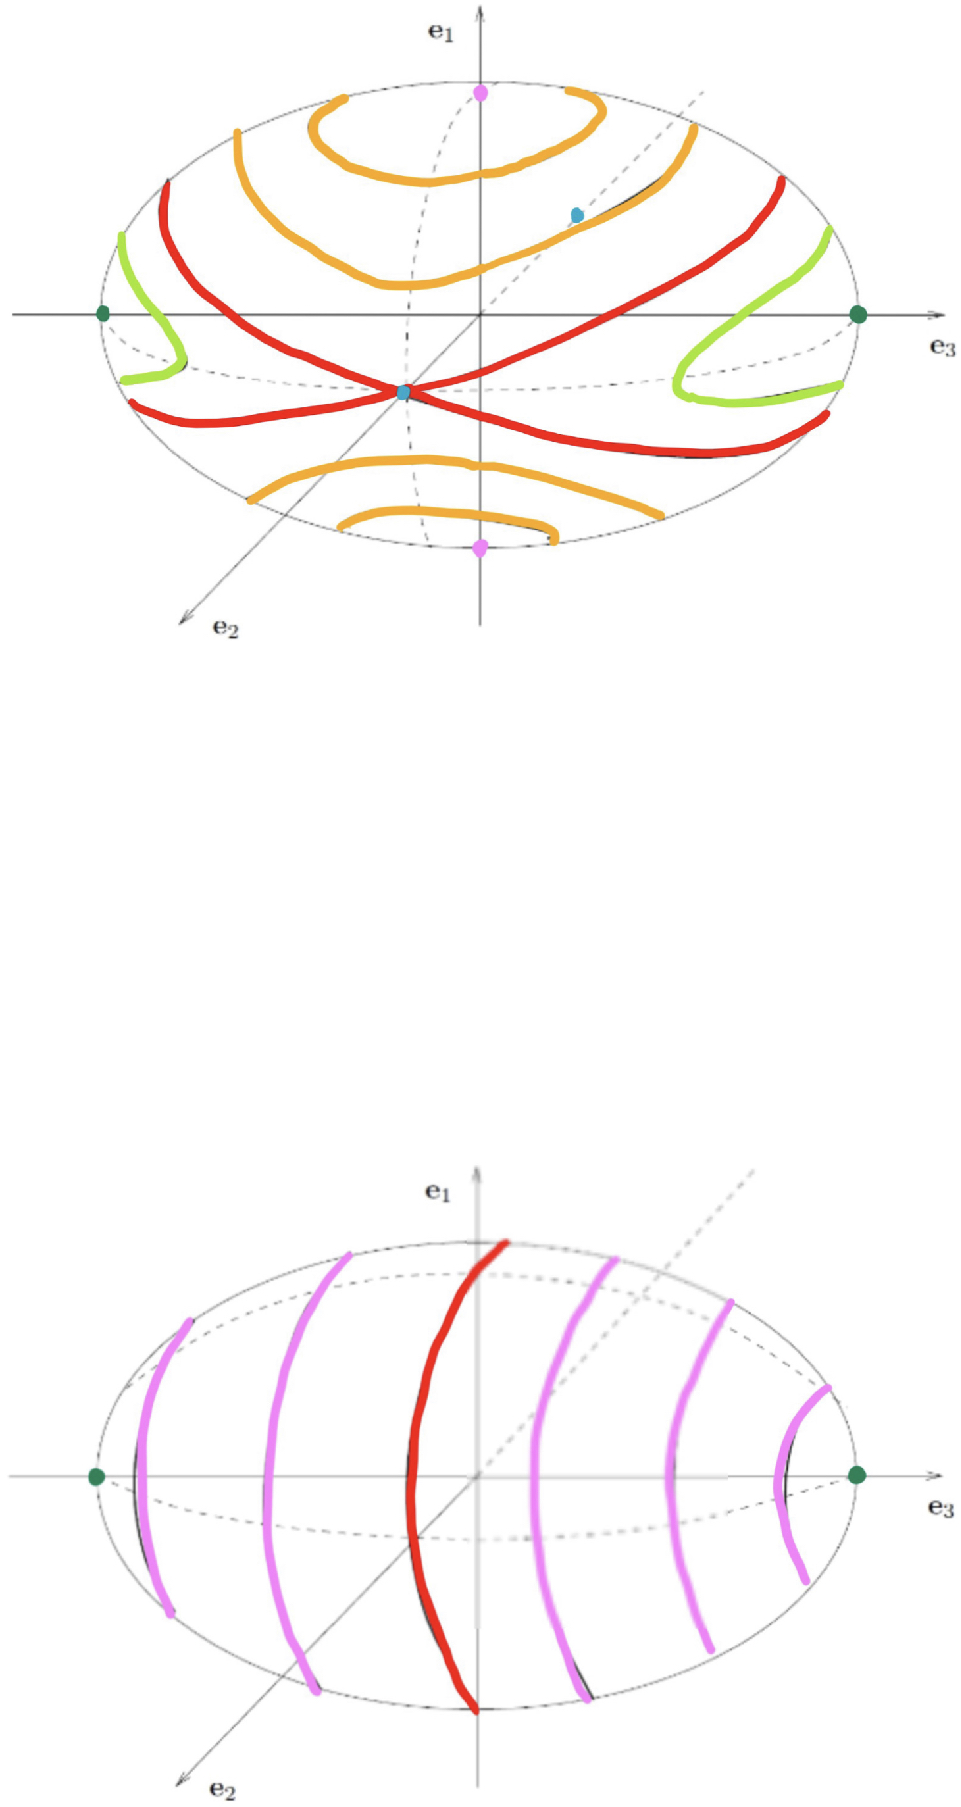
\includegraphics[width=0.23\textwidth]{MotiRL.jpeg}
\end{wrapfigure}
%
%
%
\textbf{1}]  $I_1<I_2<I_3 \ \ \text{con} \ a_i=\sqrt{2EI_i}$ \ \ \ $K\in [\sqrt{2EI_1}, \sqrt{2EI_3}]$ \\
%
%
\ • \ \ $\overline{K}=(0,0,\pm \sqrt{2EI_1}) \ e \ \overline{K}=(\pm \sqrt{2EI_3},0,0)$ sono 2 punti antipodali\\
\phantom{\ • \ \ }che generano rotazioni stazionarie,
dato che le equazioni di Eulero\\
\phantom{\ • \ \ }possiamo riscriverle $\dot{\overline{\omega}}=\overline{f}(\overline{\omega})$ allora $\omega=cost \implies$ punti di equilibrio\\ 
\ • \ \ $\overline{K}=(0,\pm \sqrt{2EI_2},0) \ e \ \overline{K}=(\pm \sqrt{2EI_1},0,0)$\\
\phantom{\ • \ \ } due punti antipodali e due circonferenze che li contengono\\
\ • \ \ $\pm \sqrt{2EI_1}< |K|<\pm \sqrt{2EI_3}$ per ogni valore di |K| ci sono due curve chiuse\\
\phantom{\ • \ \ }in un intorno dei punti antipodali più vicini \\
%
%
%
\textbf{2}] $I_1=I_2<I_3$\\
\ • \ \ $\overline{K}=(0,0,\pm \sqrt{2EI_3})$ sono 2 punti antipodali, rotazioni stazionarie\\ 
\ • \ \ $\pm \sqrt{2EI_1}< |K|<\pm \sqrt{2EI_3}$ curve chiuse\\
\ • \ \ $|K|=\sqrt{2EI_1}$ è una circonferenza di punti di equilibrio\\
Attorno ad ogni asse del piano $\hat{e}_1, \hat{e}_2$ ci sono rotazioni stazionarie\\
%
Prop: Se $I_1=I_2$ ogni soluzione delle eq di Eulero diversa dalle rotazioni stazionarie è periodica \ \ \ (+dim)\\
%
%
%
\textbf{3}] $I_1=I_2=I_3$\\
É l'intersezione tra due sfere, che genera una sfera di punti di equilibrio\\ \\
%
%
%
Teo: Se $I_1<I_2<I_3$ le rotazioni stazionarie attorno a $\hat{e}_1 \ e \ \hat{e}_3$ sono stabili, in $\hat{e}_2$ sono instabili\ \ \ (+dim) \\
%
Oss: Invece il moto del corpo rigido risulta sempre instabile, a differenza dei corrispondenti moti di $\overline{\omega}$\\
\phantom{Oss: }Perché è descritto dalla matrice di rotazione $R(t)$ che con piccole oscillazioni non rimane vicino all'asse
%
%
%Lezione28
%
\subsection{Meccanica relativa}
%
Prop: Dato un osservatore $\theta'$, la Lagrangiana di un punto materiale diventa: \\ 
\phantom{Prop: }$\mathcal{L}(\overline{q}';\dot{\overline{q}}')=\frac{1}{2}m|\dot{\overline{q}}'|^2 + m\dot{\overline{q}}'\cdot\overline{\omega}\wedge\overline{q}' + \frac{1}{2}m|\overline{\omega}\wedge\overline{q}'|^2 -m\overline{a}_{O'}\overline{q}'-U(\overline{q}')$ \ con $\overline{\omega}$ la vel angolare di $\theta'$ \ \ \ (+dim)\\
%
%
%
Esempio: Pendolo di Foucault \\
%
%
%Lezione29
%
\section{Meccanica dei Continui}

%L'obbiettivo è quello di descrivere corpi continui DEFORMABILI\\

\subsection{Deformazioni}
%
\begin{defi}
La \textbf{Configurazione di riferimento} $\mathcal{C}^*\subset \mathbb{R}^3$ di un corpo continuo (sistema meccanico continuo)\\
\phantom{DEF. } è la regione dello spazio occupata dal corpo
\end{defi}
%
Oss: Assumeremo sempre che $\partial \mathcal{C}^*$ sia sufficientemente regolare e che $\exists\rho : \mathbb{R}^3\times\mathbb{R}\rightarrow\mathbb{R}^+$ \textbf{densità di massa}\\
\phantom{Oss: }una funzione integrabile t.c.\! la massa contenuta in $\mathcal{D}\subset\mathbb{R}^3$ sia \ $m(\mathcal{D})=\int_{\mathcal{D}}\rho(\overline{x};t)d\overline{x}$ \\
%
%
%
\begin{defi}
Una \textbf{deformazione} è un diffeomorfismo ($C^1$ invertibile con inversa $C^1$) \ \ $ \overline{\chi}: \mathcal{C}^*\rightarrow \mathcal{C}$ che individua lo spostamento dei punti materiali del corpo. \
Chiameremo \textbf{deformazione inversa} \ $\overline{\Pi}:\mathcal{C}\rightarrow\mathcal{C}^*\ \ \overline{\Pi}=\overline{\chi}^{-1}$
\end{defi}
%
Oss: Le richieste sulle deformazioni derivano da ipotesi fisiche:\\
\ • \ \ $\overline{\chi} \in C^1$ perché la deformazione non può generare discontinuità (fratture)\\
\ • \ \ $\overline{\chi}$ iniettiva perché non ci può essere sovrapposizione tre due punti materiali
%
\begin{defi}
Lo \textbf{spostamento} del punto materiale $\overline{x}$ è dato da $\overline{u}(\overline{x})=\overline{\chi}(\overline{x})-\overline{x}$ \ e vale \ $\overline{u}=\overline{x}-\overline{\Pi}(\overline{x})$\end{defi}
%
%
%
\begin{defi}
Dato uno spazio vettoriale V, un tensore di ordine n su V è un’applicazione multilineare: $V^n \rightarrow \mathbb{R}$ \\
Il \textbf{gradiente di deformazione} è il tensore di secondo ordine dato dal differenziale di $\overline{\chi}$\\ ovvero la trasformazione lineare $d\overline{\chi}:\mathcal{C}^*\rightarrow\mathbb{R}^3 $ data da \ $(d\overline{\chi})_{jk}=\frac{\partial\chi_j}{\partial x_k}$
\end{defi}
Oss: Si ha quindi $\overline{\chi}(\overline{x}^*+\overline{h})=\overline{\chi}(\overline{x}^*)+d\overline{\chi}(\overline{x}^*)\overline{h} + o(\overline{h})$ per $\overline{h}\rightarrow \overline{0}$\\
%
%
%
Oss: Richiederemo sempre che $J(\overline{x}^*):=det(d\overline{\chi})(\overline{x}^*)>0 \ \forall \overline{x}^* \in \mathcal{C}$\\
Oss: É immediato dimostrare che $d\overline{\Pi}(\overline{x})=(d\overline{\chi})^{-1}(\overline{x})$\\
%
%
%
\begin{defi}
Una deformazione è \textbf{omogenea} se è t.c. $d\overline{\chi}=D$ = costante e $\overline{\chi}(\overline{x}^*)=\overline{\chi}(\overline{y}^*)+D(\overline{x}^*-\overline{y}^*)$
\end{defi}

%
Esempi di deformazioni omogenee:\\
\ • \ \ Traslazione: $D=\mathcal{I}$ \ \ \ $\overline{\chi}(\overline{x}^*)=\overline{x}^*+\overline{u} $ \\
\ • \ \ Deformazione con punto fisso, se esiste $\overline{z}^*\in\mathcal{C}^*$ t.c. $\overline{\chi}(\overline{z}^*)=\overline{z}^*$ \ \ \  $\overline{\chi}(\overline{x}^*)=\overline{z}^*+D(\overline{x}^*-\overline{z}^*)$ \\
\ • \ \ Rototralazione: $D=R\in O_3$ (R è rotazione)\ \ \  $\overline{\chi}(\overline{x}^*)=\overline{\chi}(\overline{y}^*)+R(\overline{x}^*-\overline{y}^*)$\\
\ • \ \ Rotazione è una rototraslazione con un punto fisso \ \ \  $\overline{\chi}(\overline{x}^*)=\overline{z}^*+R(\overline{x}^*-\overline{z}^*)$\\
\ • \ \ Deformazione pura: $D\in L_{sym}^+(\mathbb{R}^3)$ (operatori lineari simmetrici positivi) \\
%
\ • \ \ Stiramento di intensità $\lambda\in\mathbb{R}^+$ nella direzione $\hat{e}$ è una deformazione pura $\overline{\chi}(\overline{x}^*)=\overline{x}^*+(\lambda-1)[(\overline{x}^*-\overline{y}^*)\cdot\hat{e}]\hat{e}$\\ \\
%
Prop: Ogni deformazione omogenea $\overline{\chi}$ è ottenibile come combinazione lineare di\\
\phantom{Prop: }una deformazione con punto fisso e una traslazione\ \ \ (+dim)\\
%
Oss: Data una rotazione di asse $\hat{e}$ e punto fisso $\overline{z}^*$, i punti della retta $\overline{x}^*=\lambda\hat{e}+\overline{z}^*$ sono lasciati fissi\\
%
%
%
Prop: Date due deformazioni $\overline{\chi}_1$ e $\overline{\chi}_2$, il gradiente della composta è: \ $d(\overline{\chi}_1\circ\overline{\chi}_2)=d\overline{\chi}_1\cdot d\overline{\chi}_2$ \ \ \ (+dim)\\ \\
%
%
%
Lemma: (decomposizione polare) \ \ \ (+dim)\\
Per ogni $D\in L^+(\mathbb{R}),\ \exists!\ R \in O_3 \text{ e } U,V\in L_{sym}^+(\mathbb{R}^3)$ t.c. $D=RU=VR$ \\
%
Prop: Ogni deformazione omogenea con gradiente D è scrivibile come $\overline{\chi}=\overline{\rho}\circ\overline{\xi}_1=\overline{\xi}_2\circ\overline{\rho}$ \\
\phantom{Prop: }dove $\overline{\rho}$ è una rotazione di gradiente R e $\overline{\xi}_1, \overline{\xi}_2$ sono delle deformazioni pure di gradienti U e V \ \ \ (+dim)\\ \\
%
%
%
Oss: Per definizione e linearità del differenziale ogni deformazione è almeno localmente omogenea\\
\phantom{Oss: }e si può approssimare con una deformazione omogenea: \ $\overline{\chi}(\overline{x}^*+\overline{h})=\overline{\chi}(\overline{x}^*)+d\overline{\chi}(\overline{x}^*)\overline{h} +o(\overline{h})$ \\
%
%
%
\begin{defi}
Data una deformazione $\overline{\chi}$ i \textbf{tensori di Cauchy-Green} destro e sinistro sono rispettivamente:\\
\phantom{DEF: } $B:=d\overline{\chi}\cdot d\overline{\chi}^T \ \ C:=d\overline{\chi}^T\cdot d\overline{\chi} $
\end{defi}
%
Oss: $B,C \in L_{sym}^+(\mathbb{R}^3)$ e data la decomposizione polare $d\overline{\chi}=RU = VR$ si ha: \\
\ - \ $B=U^2 \ \ C=V^2 \ \ C=R^TBR$ \ \
\ - \ autovalori di B =autovalori di C\\
\ - \ $I_j(B)=I_j(C)\ \forall j\in \{1,2,3\}$ dove $I_j$ sono gli invarianti ortogonali \\
%
\begin{defi}
Un \textbf{invariante ortogonale} è una funzione $f:L(\mathbb{R}^3)\rightarrow\mathbb{R} \ t.c. \ f(RA)=f(A) \ \forall R\in O_3 \ e \ \forall A \in L(\mathbb{R}^3)$
\end{defi}
%
Prop: Gli invarianti ortogonali sono le funzioni: \ $I_1(A):=tr(A) \ \ \ I_2(A):=\frac{1}{2}[tr(A)^2-tr(A^2)] \ \ \ I_3(A):=det(A)$ \\
%
Oss: Il polinomio caratteristico di un tensore in $L(\mathbb{R}^3)$ si esprime come $p(\lambda)=-\lambda^3+I_1\lambda^2-I_2\lambda+I_3=0$\\
\phantom{Oss: }e in effetti per ogni $A\in L(\mathbb{R}^3)$ \ \ $-A^3+I_1(A)A^2-I_2(A)A+I_3(A)=0$\\ \\
%
%
%Lezione30
%
Oss: Il gradiente di deformazione può essere pensato come trasformazione: $\mathcal{C}^*\rightarrow\mathcal{C}$ \ \ \ $dx_i=\sum_{j=1}^3(d\overline{\chi})_{ij} dx^*_j$ \\
Oss: Allo stesso modo $d\overline{\chi}^T$ è applicazione lineare: $\mathcal{C}\rightarrow\mathcal{C}^*$ e quindi i tensori \ \ $B: \mathcal{C}\rightarrow\mathcal{C} \ e \ C: \mathcal{C}^*\rightarrow\mathcal{C}^*$\\  
%
%
%
\begin{defi}
Data una curva $\overline{\gamma}:\mathbb{R}\rightarrow\mathcal{C}^*$ t.c. $\ \ \begin{cases}
    \overline{\gamma}(s^*)=\overline{x}^*\\
    \overline{\gamma}'(s^*)=\hat{e}
\end{cases}$ \ costruiamo una curva deformata\ \ $\begin{cases}
    \widetilde{\overline{\gamma}}(s)=\overline{\chi}(\overline{\gamma}(s))\\
    \widetilde{\overline{\gamma}}'(s^*)=D\overline{\gamma}'(s^*)=D\hat{e}
\end{cases}$ \\
%
Lo \textbf{stiramento} in direzione $\hat{e}$ è
\ $\delta(\hat{e}):=\frac{d\widetilde{s}}{ds}=|D\hat{e}|$ \ \ e la \textbf{deformazione longitudinale} è $\lambda(\hat{e}) :=\delta(\hat{e})-1$
\end{defi}
%
Oss: $\delta^2(\hat{e})=\hat{e}(C\hat{e})=\hat{e}'B\hat{e}'$\\
%
%
%
Prop: (deformazione tra due punti vicini) \ \ $lim_{\varepsilon\rightarrow 0^+} \frac{|\overline{\chi}(\overline{x}^*+\varepsilon\hat{e})|^2}{\varepsilon^2}=\hat{e}C\hat{e}$ \ \ \ (+dim) \\
%
%
%
\begin{defi}
Date due curve $\overline{\gamma}_{1,2}:\mathbb{R}\rightarrow\mathcal{C}^*$ e posti $\ \ \begin{cases}
    \overline{\gamma}_i(s^*)=\overline{x}^*\\
    \overline{\gamma}_i'(s^*)=\hat{e}_i
\end{cases}$ \ \ \ $\overline{\chi}'(\overline{\gamma}_i(s^*))=d\overline{\chi}\cdot\hat{e}_i$\\
%
L'\textbf{angolo di scorrimento} è la quantità $\gamma(\hat{e}_1,\hat{e}_2):= \frac{\pi}{2}-\theta(\hat{e}_1,\hat{e}_2)$ \ \ \ dove $\theta$ è l'angolo formato tra $d\overline{\chi}\hat{e}_1 \ e \ d\overline{\chi}\hat{e}_2$
\end{defi}
%
Prop: $sen( \gamma(\hat{e}_1,\hat{e}_2))= \frac{\hat{e}_1 C \hat{e}_2}{\sqrt{\hat{e}_1 C \hat{e}_1} \sqrt{\hat{e}_2 C \hat{e}_2}}$ \ \ \ (+dim)\\
%
Oss: Le componenti di C diventeranno \ \ $C_{ii}=\delta_i^2 \ \ \ C_{ij}=\delta_i\delta_j sen(\gamma_{ij})$\\ % ci vorrebbe il doppio invio, ma finisce la pagina
%
%
%
Prop: Data una deformazione $\overline{\chi}, \ \forall\overline{x}^* \in \mathcal{C}^* \ \exists$ terna ortonormale $ \{\hat{e}_1, \hat{e}_2, \hat{e}_3\}$ t.c. C è diagonale in tale terna $C=diag\{\widetilde{\delta}^2_1, \widetilde{\delta}^2_2, \widetilde{\delta}^2_3\}$ e $\overline{\chi}$ rispetto alla terna è data da 3 stiramenti lungo gli assi, che individuano le direzioni principali di deformazione, inoltre rispetto a tale base $\widetilde{\delta}_i$ sono detti stiramenti principali \\ \\
%
Oss: Siano $\mathcal{D}^*\subset\mathcal{C}^* $ un insieme misurabile e $ \ \mathcal{D}=\{ \overline{x}\in\mathcal{C} \ | \ \exists \overline{x}^* \in \mathcal{D}^*, \ \overline{x}=\overline{\chi}(\overline{x}^*) \} $ l'insieme \\
\phantom{Oss: }trasformato, allora \ \ $ |\mathcal{D}|=\int_{\mathcal{D}^*}det(d\overline{\chi}(\overline{x}^*))d\overline{x}^*$ \\
%
Oss: Le deformazioni che non cambiano i volumi (isocore) sono tutte e sole quelle con $det(d\overline{\chi})=1 \ \forall \overline{x}^*\in\mathcal{C}^* $\\
%
Oss: Dato un campo scalare $\Phi:\mathbb{R}^3\rightarrow\mathbb{R}$ vale: \ $\int_{\mathcal{D}}\Phi(\overline{x})d\overline{x} = \int_{\mathcal{D}^*} det(d\overline{\chi}(\overline{x}^*))  \Phi(\overline{\chi}(\overline{x}^*))d\overline{x}^*$ \\
%
%
%
\begin{defi}
Data una \textbf{deformazione infinitesima}, cioè t.c. $\overline{u}(\overline{x}^*)=\overline{\chi}(\overline{x}^*) - \overline{x}^* <<1$ \\ il gradiente di deformazione infinitesimo è \ $E:=\frac12 (d\overline{u}+d\overline{u}^T)=\frac12 (d\overline{\chi} + d\overline{\chi}^T)-\mathds{1}$
\end{defi}
%
%
Oss: Data una deformazione infinitesima, abbiamo:\\
\ • \ $C=\mathds{1}+2E+O(\varepsilon^2)$ \ \ \ \ • \ $U=\mathds{1}+E+O(\varepsilon^2)$\\
\ • \ $R=\mathds{1}+d\overline{u}-E+O(\varepsilon^2)=\mathds{1}+W+O(\varepsilon^2)$ \ \ \ dove $W:=\frac12 (d\overline{u}-d\overline{u}^T)$ è la componente antisimmetrica di $d\overline{u}$\\ \\
%
Oss: Dato uno stiramento infinitesimo in direzione $\hat{e}$, abbiamo:\\
\ • \ $\delta(\hat{e})= 1 + \hat{e}E\hat{e} +O(\varepsilon^2)$ \ \ \ \ • \ $\lambda(\hat{e})=\hat{e}E\hat{e}$\ \ \ \ • \ $sen[\gamma(\hat{e}_i,\hat{e_j})]=2\hat{e}_iE\hat{e}_j + O(\varepsilon^2)$\\
\ • \ Per quanto riguarda la variazione di volume \ $d\overline{x}=det(d\overline{\chi})d\overline{x}^* \implies d\overline{x}=(1+TrE+O(\varepsilon^2))d\overline{x}^*$



\subsection{Moti}
%
\begin{defi}
La configurazione attuale è \ $\mathcal{C}_t := \overline{\chi}(\mathcal{C}^*;t)$\\
%
Un \textbf{moto} di un corpo continuo è una famiglia di deformazioni: \ $\{ \overline{\chi}(\cdot\ ,t) \}_{t\in\mathbb{R}} \ , \ \overline{\chi}(\cdot\ ;\cdot) : \mathcal{C}^*\times\mathbb{R}\rightarrow \mathcal{C}_t $ \\
La \textbf{traiettoria} di un punto materiale $\overline{x}^*$ è $\overline{x}(t) := \overline{\chi}(\overline{x}^*;t)$ \\
La traiettoria del sistema è $\mathcal{C}_{\overline{x}}=\{ (\overline{x},t)\in\mathbb{R}^3\times\mathbb{R} \ |\ \exists\ \overline{x}^*\in \mathcal{C}^* , \overline{x}=\overline{\chi}(\overline{x}^*,t) \}=\{\mathcal{C}_t\}_{t\in\mathbb{R}}$
\end{defi}
%
%
La velocità e l'accelerazione di $\overline{x}^*$ al tempo t sono: \ $\dot{\overline{x}}=\frac{\partial}{\partial t}\overline{\chi}(\overline{x}^*;t) \ \ \ \Ddot{\overline{x}}=\frac{\partial^2}{\partial t^2} \overline{\chi}(\overline{x}^*;t)$\\
%
Oss: Assumeremo sempre che $\overline{\chi}$ sia $C^2$ nei suoi argomenti \\ \\
%
%
%
Oss: L'invertibilità di $\overline{\chi}$ garantisce che 
$\forall t \ \exists \overline{\Pi}: \mathcal{C}_t\rightarrow\mathcal{C}^* \ \ t.c. \ \ \overline{\Pi}(\overline{\chi}(\overline{x}^*;t);t)=\overline{x}^* \ e \ \overline{\chi}(\overline{\Pi}(\overline{x};t);t)=\overline{x}$\\
%
Oss: Posso vedere lo spostamento in due modi:\\
\phantom{Oss: }1) Descrizione Lagrangiana o materiale, prendendo i punti e studiandone l'evoluzione nel tempo\\
\phantom{Oss: }2) Descrizione Euleriana o spaziale, fissando il tempo e studiando velocità e accelerazione per ogni punto\\
\phantom{Oss: 2) }$\overline{v}(\overline{x};t)=\dot{\overline{x}}(\overline{\Pi}(\overline{x};t),t)$ \ \ \ $\overline{a}(\overline{x};t)=\ddot{\overline{x}}(\overline{\Pi}(\overline{x};t),t)$ \\ \\
%
%
%Lezione31
%
Campo spaziale \ $\overline{\Phi}:\mathcal{C}_t\times\mathbb{R}\rightarrow\mathbb{R}^n \ \ \overline{\Phi}(\overline{x};t)$ \ \ \
Campo materiale \ $\overline{\Psi}:\mathcal{C}^*\times\mathbb{R}\rightarrow\mathbb{R}^n \ \ \overline{\Psi}(\overline{x}^*;t)$\\
%
%
%
Oss: É sempre possibile passare da un campo all'altro:\ \ $\overline{\Phi}_m(\overline{x}^*;t):= \overline{\Phi}(\overline{\chi}(\overline{x}^*;t),t) \ \ \ \overline{\Psi}_s(\overline{x};t):= \overline{\Psi}(\overline{\Pi}(\overline{x},t);t)$\\ \\
%
%
%
Prop: Indicando con $\dot{\overline{x}}, \ddot{\overline{x}}$ e $\overline{v},\overline{a}$ rispettivamente i campi materiali e spaziali di velocità e accelerazione\\
\phantom{Prop: }si ha, \ \ $d_*\dot{\overline{x}}=d\overline{v}\ d_*\overline{\chi}= d\dot{\overline{\chi}} \ \ \ d_*\ddot{\overline{x}}=d\overline{a}\ d_*\overline{\chi}= d\ddot{\overline{\chi}}$ \ \ \ (+dim)\\
%
Oss: Dove i gradienti $d \ e \ d_*$ sono calcolati rispetto a coordinate diverse, rispettivamente $\overline{x} \ e \ \overline{x}^*$ \\
%
Oss: Di conseguenza valgono\ \ \ $d\overline{v}=d\dot{\overline{\chi}}d\overline{\chi}^{-1} \ \ \ d\overline{a}=d\ddot{\overline{\chi}}d\overline{\chi}^{-1}$\\ \\
%
%
%
Oss: Posti \ \ \ $(d_*\overline{\Psi})_{ij}=\frac{\partial \Psi_i}{\partial x^*_j} \ \ \ (d\overline{\Phi})_{ij}=\frac{\partial \Phi_i}{\partial x_j}$, \ \ \ è ovvio che \ $d_*\overline{\Psi}=d\overline{\Psi}_sd_*\overline{\chi} \ \ e \ \ d\overline{\Phi}=d_*\overline{\Phi}_md\overline{\chi}^{-1}$ \\
%
%
Oss: Analogamente per divergenze \ \ $\nabla_*\cdot\overline{\Psi}:=tr(d_*\overline{\Psi}) \ \ \ \nabla\cdot\overline{\Phi}:=tr(d\overline{\Phi}) $\\ \\
%
%
%
Oss: Per i campi spaziali vale\ \ $\dot{\overline{\Phi}}(\overline{x};t) = d\overline{\Phi}\cdot\overline{v} + \frac{\partial\overline{\Phi}}{\partial t}$ \ e in particolare per l'accelerazione \ $\overline{a}(\overline{x};t)= d\overline{v}\cdot\overline{v} + \frac{\partial\overline{v}}{\partial t}$\\
%
%
%
\begin{defi}
Un campo spaziale è \textbf{stazionario} se $\frac{\partial \overline{\Phi}}{\partial t}=0$ per $t \in [t_0,t_1]$
\end{defi}
%
Oss: Associate alla doppia descrizione materiale e spaziale del moto, abbiamo una doppia tipologia di curve\\
\phantom{Oss: }• Linee di corrente che descrivono le traiettorie dei singoli punti materiali \ \ $\overline{x}(t)=\overline{\chi}(\overline{x}^*;t)$ \\
\phantom{Oss: }• Linee di flusso che fissato il tempo, sono tangenti in ogni punto al campo di velocità \ $\overline{x}'(s)=\overline{v}(\overline{x}(s);t)$\\
%
Oss: Se il campo spaziale delle velocità è stazionario allora le linee di flusso coincidono con le linee di corrente \\
%
%
%
\begin{defi}
Dato un campo spaziale di velocità, il suo gradiente si decompone \ $d\overline{v}=D+W$\\
$D=\frac{1}{2}(d\overline{v}+d\overline{v}^t)$ è il tensore di \textbf{deformazione di velocità} e $ \ W=\frac{1}{2}(d\overline{v}-d\overline{v}^t)$ è il tensore di \textbf{vorticità}
%
\end{defi}
Oss: Poiché W è antisimmetrica, $\exists \overline{w}\in \mathbb{R}^3$ (vorticità) t.c. $\forall \overline{u}\in\mathbb{R}^3 \ \ W\overline{u}=\frac{1}{2}\overline{w}\wedge\overline{u} \ \ \ \ \overline{w}=\nabla\wedge\overline{v}$\\ \\
%
%
%
Teo: Il moto di un campo continuo è rigido $\Longleftrightarrow D=0$ \ \ \ (+dim)\\ \\
%
%
%
Prop: Fissato un versore $\hat{e}$ si ha $\frac{\dot{\delta}(t)}{\delta(t)}=\hat{e}D\hat{e}$ \ dove $\dot{\delta}(t)$ è la velocità di stiramento in direzione $\hat{e}$ \ \ \ (+dim)\\
%
%
%
Prop: Dati due versori $\hat{e}_1, \hat{e}_2$ perpendicolari si ha $\dot{\theta}(t)=-2\hat{e}_1D\hat{e}_2$ dove $\dot{\theta}$ è la velocità di scorrimento \ \ \ (+dim) \\ \\
%
%
%Lezione32
%
Prop: Sia $\mathcal{D}_t\in\mathcal{C}_t$ misurabile, allora \ $\frac{d}{dt}|\mathcal{D}_t|=\int_{\mathcal{D}_t}\nabla\cdot\overline{v}\ d\overline{x}$ \ \ \ (+dim)\\
%
Lemma: Sia T(t) un tensore derivabile e invertibile $\forall t \in \mathbb{R}$ \ allora $\dot{(det T(t))} = det T\cdot tr(\dot{T}T^{-1})$ \ \ \ (+dim)\\
%
Oss: Il volume di un continuo è conservato (incomprimibilità) $\Leftrightarrow \nabla\cdot\overline{v}=0$ \\
\phantom{Oss: } Quindi \ D=0 $\Leftrightarrow$ continuo rigido \ \ e \ $trD=0$ $\Leftrightarrow$ incomprimibilità\\ \\
%
%
%
Teo (Trasporto di Reynolds) \ \ \ (+dim)\\
Siano $\overline{\Phi}(\overline{x},t)$ un campo spaziale regolare e $\mathcal{D}_t\subset\mathcal{C}_t$ con bordo regolare, allora \\ $\frac{d}{dt}\int_{\mathcal{D}_t}\overline{\Phi}(\overline{x},t)d\overline{x} = \int_{\mathcal{D}_t}\frac{\partial \overline{\Phi}}{\partial t}(\overline{x},t)d\overline{x} + \int_{\partial \mathcal{D}_t}\overline{v}\cdot\hat{n} \ \overline{\Phi}(\overline{x},t)d\overline{\sigma}$ \ \ \ dove $\hat{n}$ è la normale uscente da $\mathcal{D}_t$



\subsection{Leggi di bilancio}
%
Dato un corpo continuo, esistono misurabili le funzioni massa:\\
%
$\exists\ \rho^*: \mathcal{C}^*\rightarrow  \mathbb{R}^+ \ \ \ m(\mathcal{D}^*)=\int_{\mathcal{D}^*}\rho^*(\overline{x}^*)d\overline{x}^* $\\
$\exists\ \rho(\overline{x},t):\mathcal{C}_t\rightarrow\mathbb{R}^+ \ \ m(\mathcal{D}_t)= \int_{\mathcal{D}_t}\rho(\overline{x},t)d\overline{x} $ \\
%
Prop: La massa contenuta in ciascuna parte del continuo è conservata se e solo se\\
\phantom{Prop: }$\rho_t=det(d\overline{\chi})\rho_m$ \ \  dove $\rho_m$ è il campo materiale associato a $\rho$ \ \ \ (+dim)\\
%
Lemma (di localizzazione): \ \ \ (+dim)\\
Sia $\overline{\Phi}:\mathcal{C}\rightarrow\mathbb{R}^m$ continuo t.c. $\int_{\mathcal{D}}\overline{\Phi}(\overline{x})d\overline{x}=\overline{0} \ \ \forall \mathcal{D}\subset \mathcal{C}$ misurabile $\ \implies \overline{\Phi}=0$ in $\mathcal{C}$ \\ \\
%
%
%
Teo: La massa di un continuo è conservata lungo il moto se e solo se vale l'equazione di continuità  \\
\phantom{Teo: }$\frac{d\rho}{dt} + div(\rho\overline{v})=0$ \ \ \ (1° legge di bilancio) \ \ \ (+dim)\\
%
%
%
Cor: $\forall \overline{\Phi}$ campo spaziale regolare e $\forall \mathcal{D}_t\subset\mathcal{C}_t$ misurabile ho che $\frac{d}{dt}(\int_{\mathcal{D}_t}\rho\overline{\Phi}d\overline{x})=\int_{\mathcal{D}_t}\rho\frac{d}{dt}\overline{\Phi}d\overline{x}$ \ \ \ (+dim)\\
%
Oss: Incomprimibilità $\implies \frac{\partial \rho}{\partial t} + \overline{v}\cdot\nabla\rho=0$\\
%
%
%
\begin{Ndefi}
Quantità meccaniche per un continuo sono: \ \ $\overline{Q}=\int_{\mathcal{C}_t}\rho(\overline{x};t)\overline{v}d\overline{x} \ \ \ \ \overline{K}_0=\int_{\mathcal{C}_t}(\overline{x}-\overline{x}_0)\wedge\overline{v}\ \rho(\overline{x};t)d\overline{x}$\\
%
Forze (esterne): \\ • di volume se $\exists \overline{f}_v(\overline{x},t) \ t.c. \ \overline{F}(\mathcal{D}_t)=\int_{\mathcal{D}_t}\overline{f}_v(\overline{x},t)d\overline{x}$ \ \ \
• di superficie se $\exists \overline{f}_s(\overline{x},t) \ t.c. \ \overline{F}(\Sigma_t)=\int_{\Sigma_t}\overline{f}_s(\overline{x},t)d\overline{\sigma}$\\
%
%
%
Forze (interne), ipotesi di Cauchy:\\
$\exists$ una densità superficiale di forza $\overline{f}_{s,int}(\overline{x},\hat{n})$ t.c. la forza esercitata da $\mathcal{C}^+_t \ a \ \mathcal{C}^-_t$ sia $\overline{F}_{+-}=\int_{\Sigma}\overline{f}_{s,int}(\overline{x},\hat{n}(\overline{x}))d\overline{x}$
\end{Ndefi}
%
%
%
Teo: (Cauchy) \ \ \ (+dim)\\
Siano $\overline{\Phi}(\overline{x})$ e $\overline{S}(\overline{x},\hat{n})$ due campi spaziali continui sui loro argomenti $\overline{x}\in\mathcal{C}_t \ e \ \hat{n}\in\mathcal{N}$ t.c.\\
$\int_{\mathcal{D}_t}\overline{\Phi}(\overline{x})d\overline{x} + \int_{\partial\mathcal{D}_t}\overline{S}(\overline{x};\hat{n}(\overline{x}))d\overline{\sigma}=0\ \ \forall\mathcal{D}_t\subset\mathcal{C}_t$ \ \ allora $\exists$ tensore $T(\overline{x})$ t.c. $\overline{S}(\overline{x};\hat{n})=T(\overline{x})\hat{n}$\\
%
Oss: Il teorema di Cauchy è una manifestazione del principio di azione e reazione, perché \ $\overline{S}(\overline{x};-\hat{n})=-\overline{S}(\overline{x};\hat{n})$ \\ \\
%
%
%Lezione33
%
Teo: Per ogni continuo, valgono: \ \ \ (+dim)\\
i) $\exists T(\overline{x};t)\in L(\mathbb{R}^3)$ \textbf{tensore degli sforzi} t.c. $\overline{f}_s(\overline{x};\hat{n};t)=T(\overline{x},t)\hat{n}$\\
ii) I eq indefinita \ \ $divT + \overline{f}_v=\rho\overline{a}$\\
iii) II eq indefinita \ \ $T=T^t$\\
%
%
Oss: $divT(\overline{x};t):=tr(dT(\overline{x};t))$\\
%
Oss: T deve soddisfare le condizioni al contorno $T(\overline{x},t)\hat{n}(\overline{x})=\overline{f}_s(\overline{x},\hat{n}(\overline{x}),t) \ \ \forall\overline{x}\in\partial\mathcal{C}_t$ \\
\phantom{Oss: }con $f_s$ la densità di forze esterne agenti su $\partial\mathcal{C}_t$\\ \\
%
%
%
Oss: $T(\overline{x})$ permette di calcolare la forza agente sulle superfici del corpo passanti per $\overline{x}$\\
%
%
%
Oss: Per applicare il teorema di Cauchy abbiamo assunto che $\rho, \overline{a}, \overline{f}_v\ e\ \overline{f}_s$ siano campi continui\\
%
%
%
Oss: T simmetrica $\implies \sum_{j=1}^3\hat{e}_j\wedge(T\hat{e}_j)=\overline{0}$ \\ \\
%
%
Oss: La distribuzione superficiale di forza agente su $\Sigma$ è $T(\overline{x})\hat{n}(\overline{x})$ con $\hat{n}$ normale uscente da $\Sigma$ \\
%
\phantom{Oss: } ma non è detto che sia $\parallel \hat{n}(\overline{x})$
%
\begin{defi}
Si diranno sforzo normale $\overline{S}_n=(\hat{n}T\hat{n})\hat{n}$ e sforzo di taglio $\overline{S}_{\tau}=T\hat{n}-\overline{S}_n$
\end{defi}
%
%
Oss: $\forall \overline{x}\in\mathcal{C}_t \ \exists \hat{e}_1,\hat{e}_2,\hat{e}_3$ t.c. le superfici $\perp \hat{e}_j$ in $\overline{x}$ sono soggette solo a sforzi normali\\
\phantom{Oss: }Gli $\hat{e}_j$ sono gli autovettori di $T(\overline{x})$ e sono detti direzioni principali di sforzo\\ 
\phantom{Oss: }i valori corrispondenti (autovalori di $T(\overline{x})$) sono detti sforzi principali\\
%
%
%
Oss: Quindi le equazioni del moto per un continuo sono \ \ $\begin{cases}
\frac{\partial\rho}{\partial t} +div(\rho\overline{v})=0\\
\rho(\frac{\partial\overline{v}}{\partial t} + \overline{v}\cdot d\overline{v})=\overline{f}_v+divT\\
\sum_{j=1}^3\hat{e}_j\wedge(T\hat{e}_j)=\overline{0}
\end{cases}$\\
\phantom{Oss: }Vanno aggiunte le condizioni iniziali: \ $\rho(\overline{x},0)=\rho_0(\overline{x}) \ \ \ \overline{v}(\overline{x},0)=\overline{v}_0(\overline{x})$ \\
\phantom{Oss: }e quelle al contorno: \ $ T(\overline{x},t)\hat{n}(\overline{x},t)=\overline{f}_{s,ext}(\overline{x},t) \ \ \forall \overline{x}\in\partial\mathcal{C}_t$ \\
Oss: In totale avrò 10 incognite, ma solo 4 equazioni




\subsection{Classi costitutive}
%
Oss: É necessario specificare le proprietà del continuo, ovvero fornire relazioni costitutive della risposta\\
\phantom{Oss: }del continuo a sollecitazioni esterne e quindi la dipendenza di T da $\rho \ e \ \overline{v}$\\
Oss: Delle possibili restrizioni possono essere:\\ 
\phantom{Oss: }• invarianza rispetto al cambio di osservatore \ \ • simmetrie del continuo \ \ • vincoli interni
%
\begin{defi}
Un \textbf{fluido} è un continuo t.c. all'equilibrio lo sforzo di taglio è sempre nullo $\overline{S}_{\tau}=\overline{0}$\\
Per ogni fluido all'equilibrio $\exists$ campo spaziale $p(\overline{x})$ chiamato di \textbf{pressione idrostatica} t.c. $T(\overline{x})=-p(\overline{x})\mathds{1}$\\
%
Un \textbf{fluido perfetto} è un continuo t.c. $\exists p(\overline{x},t) $ campo di pressione $ \ t.c. \ T(\overline{x},t)=-p(\overline{x},t)\mathds{1}$
\end{defi}
%
Oss: Per un fluido all'equilibrio il campo delle velocità è stazionario $\frac{\partial \overline{v}}{\partial t}=\overline{0}$\\
%
%
%
Prop: Un fluido è all'equilibrio $\Longleftrightarrow\nabla \wedge \overline{f}_v=\overline{0}$, in tal caso le eq indefinite si riducono alle\\ \phantom{Prop: }equazioni di Stevino: \ 
$\begin{cases} \frac{\partial}{\partial t}\rho+div(\rho\overline{v})=0 \\ \nabla p=\overline{f}_v \end{cases}$\ \ \ (+dim)\\ \\
%
%
%
Oss: Rimangono 5 incognite e 4 equazioni, quindi per chiudere le eq del moto di un fluido all'equilibrio\\
\phantom{Oss: }É necessario aggiungere una relazione costitutiva \ $\Phi(\rho,p)=0$\\
\ • \ \ $p=p(\rho) \text{ e } div(v)=0$, cioè p costante e fluido incomprimibile\\
\ • \ \ $p=K\rho$ gas perfetto isotermo\\
\ • \ \ $p=K\rho^{\gamma}$ gas perfetto adiabatico\\ \\
%
%
Oss: Per un fluido stazionario la condizione al contorno diventa $\ -p(\overline{x})\hat{n}(\overline{x})=\overline{f}_{s,ext}(\overline{x}) \ \ \forall \overline{x}\in \partial \mathcal{C}_t$\\
%
%Lezione34
%
Oss: Per fluidi perfetti le condizioni al contorno diventano
$\overline{v}\cdot\hat{n}=0 \ \forall \overline{x}\in\partial \mathcal{C}_t$\\
%
%
%
Oss: Per i fluidi perfetti le equazioni sono \ \ $\begin{cases}
\frac{\partial \rho}{\partial t} + div(\rho\overline{v})=0 \\
\rho(\frac{\partial\overline{v}}{\partial t} +\overline{v}\cdot d\overline{v}) +\nabla p=\overline{f}_v  \end{cases}$\\ \\
%
Oss: Se inoltre i fluidi perfetti sono incomprimibili e omogenei $\implies$ densità costante $\rho(\overline{x},t)=\rho=cost$\\
\phantom{Oss: }le equazioni diventano le eq di Eulero \ \ $\begin{cases}div(\overline{v})=0 \\ \frac{\partial\overline{v}}{\partial t} +\overline{v}\cdot d\overline{v} +\frac{\nabla p}{\rho}=\frac{\overline{f}_v}{\rho} \end{cases}$ \ \ $\overline{f}$ è la forza per unità di massa\\ \\
%
%
%
Teo: (Bernoulli) \ \ \ (+dim)\\
Dato un fluido perfetto, incomprimibile e omogeneo se il campo $\overline{v}$ è stazionario e le forze di volume sono conservative, allora la quantità $E=\frac{1}{2}|\overline{v}|^2+\frac{p}{\rho}+\frac{U}{\rho}$ è costante lungo le linee di flusso \\
%
Lemma: \ $\overline{v}\cdot d\overline{v}=\frac{1}{2}\nabla|\overline{v}|^2 -\overline{v}\wedge(\nabla\wedge\overline{v})$ \ \ \ (+dim)\\
%
%
%
\begin{defi}
Fluido \textbf{newtoniano}, o \textbf{viscoso}, è un continuo con relazione costitutiva: $\ T=-p\mathds{1} + \lambda div(\overline{v})\mathds{1}+2\mu D$\\
dove $\lambda, \mu >0$ sono i coefficienti di viscosità e D è il tensore di velocità di deformazione $D=\frac{1}{2}(d\overline{v}+d\overline{v}^t)$
\end{defi}
%
Prop: Le equazioni del moto di un fluido newtoniano sono le equazioni di Navier-Stokes\ \ \ (+dim)\\
\phantom{Prop: }$\begin{cases}
\frac{\partial\rho}{\partial t} + div(\rho\overline{v})=0\\
\rho(\frac{\partial\overline{v}}{\partial t}+\overline{v}\cdot d\overline{v}) -(\lambda+\mu)\nabla div(\overline{v}) -\mu\Delta\overline{v} +\nabla p = \overline{f}_v
\end{cases}$ \\
%
Oss: Le condizioni al contorno tipiche sono "no slip", cioè la velocità relativa tra fluido e contenitore è nulla\\

















\end{document}